%% 
%% Copyright 2019-2024 Elsevier Ltd
%% 
%% This file is part of the 'CAS Bundle'.
%% --------------------------------------
%% 
%% It may be distributed under the conditions of the LaTeX Project Public
%% License, either version 1.3c of this license or (at your option) any
%% later version.  The latest version of this license is in
%%    http://www.latex-project.org/lppl.txt
%% and version 1.3c or later is part of all distributions of LaTeX
%% version 1999/12/01 or later.
%% 
%% The list of all files belonging to the 'CAS Bundle' is
%% given in the file `manifest.txt'.
%% 
%% Template article for cas-sc documentclass for 
%% double column output.

\documentclass[a4paper,fleqn]{cas-sc}

% If the frontmatter runs over more than one page
% use the longmktitle option.

%\documentclass[a4paper,fleqn,longmktitle]{cas-sc}

%\usepackage[numbers]{natbib}
%\usepackage[authoryear]{natbib}
\usepackage[authoryear,longnamesfirst]{natbib}

% Revision markup (reviewer response, PHYSA-263545): \add{} = added text (red), \del{} = deleted
% text (red strikethrough). Remove before final submission. \sout cannot wrap a whole \footnote,
% table, or float: mark up their contents, or comment the float out and leave a \del{} note.
\usepackage{xcolor}
\usepackage[normalem]{ulem}
\newcommand{\add}[1]{\textcolor{red}{#1}}
\newcommand{\del}[1]{\textcolor{red}{\sout{#1}}}

% cas-sc auto-loads stfloats, which enforces strict float ordering (needed
% for full-width floats in two-column layouts). Combined with this doc's
% large figures, that makes any figure that can't fit "here"/"top"/"bottom"
% block every later float behind it, and without intervention the last two
% figures drift all the way past the bibliography to the very last page.
% A single plain \clearpage before the Conclusion (see below) fixes it,
% and needs no extra package.
% Dedicated float pages otherwise use infinitely stretchy glue
% (\@fptop/\@fpsep/\@fpbot) to spread floats out and fill the page height --
% this is what causes large blank gaps above/below/between figures on
% float-only pages. Fixed (non-stretchy) values pack them tightly instead.
\makeatletter
\setlength{\@fptop}{0pt}
\setlength{\@fpsep}{8pt}
\setlength{\@fpbot}{0pt}
\makeatother

%%%Author macros
\def\tsc#1{\csdef{#1}{\textsc{\lowercase{#1}}\xspace}}
\tsc{WGM}
\tsc{QE}
%%%

% Uncomment and use as if needed
%\newtheorem{theorem}{Theorem}
%\newtheorem{lemma}[theorem]{Lemma}
%\newdefinition{rmk}{Remark}
%\newproof{pf}{Proof}
%\newproof{pot}{Proof of Theorem \ref{thm}}

\begin{document}
\let\WriteBookmarks\relax
% Bias float placement toward staying near their in-text reference (mixed
% text+figure pages) rather than drifting to dedicated float-only pages.
\renewcommand{\topfraction}{0.9}
\renewcommand{\bottomfraction}{0.8}
\renewcommand{\textfraction}{0.07}
\renewcommand{\floatpagefraction}{0.7}

% Short title
\shorttitle{Learning dynamics as a heterogeneous cellular automaton}    

% Short author
\shortauthors{Sy et al.}  

% Main title of the paper
\title [mode = title]{Learning dynamics as a heterogeneous cellular automaton: comparing broadcast and nearest-neighbor interaction regimes in a classroom model}  

% Title footnote mark
% eg: \tnotemark[1]
% \tnotemark[1] 

% Title footnote 1.
% eg: \tnotetext[1]{Title footnote text}
% \tnotetext[1]{} 

% First author
%
% Options: Use if required
% eg: \author[1,3]{Author Name}[type=editor,
%       style=chinese,
%       auid=000,
%       bioid=1,
%       prefix=Sir,
%       orcid=0000-0000-0000-0000,
%       facebook=<facebook id>,
%       twitter=<twitter id>,
%       linkedin=<linkedin id>,
%       gplus=<gplus id>]

\author[1]{Clarence Ioakim T. Sy}
\credit{Software, Visualization, Writing - original draft}

\author[2]{Ranzivelle Marianne L. Roxas-Villanueva}
\credit{Conceptualization, Data curation, Resources, Supervision, Writing - review \& editing}

\author[1]{Johnrob Y. Bantang}
\cormark[1]
\ead{jybantang@up.edu.ph}
\credit{Conceptualization, Methodology, Formal analysis, Supervision, Writing - review \& editing}

\cortext[1]{Corresponding author}

\affiliation[1]{
    organization={National Institute of Physics, University of the Philippines Diliman},
    city={Quezon City},
    country={Philippines}}

\affiliation[2]{
    organization={Institute of Physics, University of the Philippines Los Ba\~{n}os},
    city={Laguna},
    country={Philippines}}

% For a title note without a number/mark
%\nonumnote{}

% Here goes the abstract
\begin{abstract}
  We present a probabilistic cellular automata (pCA) model to investigate the spatio-temporal learning dynamics of a classroom as a binary-state, heterogeneous agent system. Two interaction topologies are compared: a broadcast (mean-field-like) regime corresponding to traditional instruction (TI), and a nearest-neighbor coupling regime corresponding to peer instruction (PI). We characterize system behavior through the total relaxation time $t_{\rm max}$ as a function of lattice side length $L$, learning rate heterogeneity $\delta\lambda$ about a fixed mean learning rate, and spatial coupling strength $\rho_0$. In the broadcast regime, strong heterogeneity ($\delta\lambda \to 0.5$) produces a two-stage relaxation: a fast initial stage driven by high-$\lambda$ agents, followed by a slow residual stage governed by the low-$\lambda$ subpopulation. The nearest-neighbor regime is more robust to heterogeneity, exhibiting a more uniform relaxation curve with only a gradual shift in onset and, at the strongest heterogeneity, a slower final approach to the fully learned state, a behavior attributable to local propagation dynamics.  The broadcast regime has the shorter total relaxation time for larger lattice side lengths at low heterogeneity $\delta\lambda$, and the nearest-neighbor regime for smaller lattice side lengths and at high heterogeneity, where its lead in absolute time is much larger. The time for $95\%$ of agents to learn, however, is shorter in the broadcast regime over most of the parameter range for the larger lattice side length: within the model, broadcast coupling brings most agents to the learned state sooner, while nearest-neighbor coupling leaves fewer agents far behind. We further analyze the fixed-point structure of the learning dynamics via a return map, from which class-level Hake gains are approximated. The nearest-neighbor regime yields a gain function consistent with existing theoretical predictions, while the broadcast regime yields an approximately constant gain. Results are compared against empirical classroom data: at the class level, the empirical Hake gain increases with the pre-test score, consistent with the nearest-neighbor gain shape, while score decreases and the empirical seating-arrangement ranking are not reproduced.
\end{abstract}

% Use if graphical abstract is present
%\begin{graphicalabstract}
%\includegraphics{}
%\end{graphicalabstract}

% Research highlights
\begin{highlights}
\item pCA model of classroom learning under broadcast and nearest-neighbor topologies
\item Two-stage relaxation in heterogeneous broadcast systems; absent in local coupling
\item Local coupling is robust to heterogeneity through local propagation
\item Return-map fits give the Hake gain shape of each interaction regime
\end{highlights}

% Keywords
% Each keyword is seperated by \sep
\begin{keywords}
cellular automata \sep complex systems \sep opinion dynamics \sep 
heterogeneous agents \sep local propagation dynamics \sep learning dynamics
\end{keywords}

\maketitle

% Main text
\section{Introduction}\label{sec:intro}

Cellular automata (CA) models have become a well-established framework for studying the emergence of collective behavior in spatially extended systems of interacting agents~\citep{kari2005catheory, zaitsev2017generalized, louis2018probabilistic, Batac2009, arciaga2009experimental}.
Their discrete, lattice-based structure makes them particularly well-suited for capturing local interaction rules that give rise to complex macroscopic dynamics, properties exploited across a broad range of applications from epidemic spreading~\citep{Beauchemin2005} to opinion formation and social dynamics~\citep{castellano2009statistical}.
A common thread across these systems is the interplay between local and global coupling: whether agents interact primarily with their immediate neighbors or receive information from a broadcast source shapes the relaxation behavior of the system in fundamentally different ways.
This distinction, between nearest-neighbor and mean-field-like interaction topologies, is generally understood to give rise to qualitatively different dynamical regimes across a variety of spatially extended systems.

A key variable in such systems is the degree of agent heterogeneity: the spread in individual agent parameters such as coupling strength or response rate.
The degree of agent heterogeneity and local interaction environment have both been shown to significantly affect emergent collective dynamics in spatially explicit CA and agent-based models~\citep{lopez2014addressing, brown2006effects, jiao2011emergent}.
The spatial arrangement of agents and the reach of their interactions further shape these dynamics, as the neighborhood structure of the lattice directly governs the propagation pathways available to the system~\citep{dong2021influence, kari2005catheory}.
These considerations have been explored in the context of social systems, where CA-based models have demonstrated that interaction topology can be as significant as intrinsic agent parameters in determining system-level outcomes~\citep{bordogna2001theoretical, bordogna2003simulation, castellano2009statistical}.

The classroom provides a concrete and well-defined instantiation of such a heterogeneous agent system.
Students occupy fixed spatial positions on a lattice, interact with neighbors under rules governed by individual learning rates, and are subject to either a broadcast information source or local peer interaction.
Prior work by Bordogna and Albano~\citep{bordogna2001theoretical, bordogna2003simulation} demonstrated that CA-based models can capture essential features of classroom learning, including the influence of peer interaction and group structure on student outcomes.
Statistical-physics approaches have since been applied to other aspects of the teaching--learning process, including the growth of knowledge~\citep{ormazabal2021agent, velasquez2021knowledge}, sociocognitive dynamics~\citep{koponen2017modelling}, and entropy-based measures of class performance~\citep{singh2009entropic}.

Existing models of classroom learning leave open how agent heterogeneity and interaction topology act together.
Models of the Hake gain~\citep{hake1998, pritchard2008mathematical, nitta2019mathematical} describe how class-level scores change between assessments without specifying which students interact, so they cannot distinguish one interaction topology from another.
Agent-based models of the classroom~\citep{bordogna2001theoretical, bordogna2003simulation, ormazabal2021agent, velasquez2021knowledge} include students who differ in prior achievement, attention, or aptitude, and some compare lectures alone with lectures supplemented by group work~\citep{bordogna2001theoretical, ormazabal2021agent}.
In these models, however, peers interact within small groups or clusters formed without a spatial arrangement, and group work supplements the lecture rather than replacing it, so broadcast and local interaction are not compared as alternatives.
Studies of seating~\citep{roxas2010seating, monterola2009} address the spatial placement of students, and our earlier proceeding~\citep{SelfSPP} compared broadcast and nearest-neighbor coupling on a lattice, but with identical agents.
Outside the classroom, local and mean-field coupling are known to produce different spreading dynamics, for example in the diffusion of innovations~\citep{fuks1997cellular}, again for identical agents.
It therefore remains unknown how heterogeneity in learning rates interacts with the interaction topology on a spatial lattice: whether it affects broadcast and local coupling differently, how the resulting relaxation times depend on system size, and how long the slowest agents are left behind.
We address this question with a bottom-up model in which the class-level dynamics follow from the interaction rules rather than being postulated; the correspondence between model quantities and classroom observables is an interpretive choice, which we state explicitly.

We present a probabilistic cellular automata (pCA) model in which each agent is assigned a binary state and an individual learning rate $\lambda$, drawn from a two-level heterogeneous distribution parameterized by $\delta\lambda$.
Two interaction regimes are implemented and compared: a broadcast regime in which each agent updates independently based on a global source, and a nearest-neighbor regime in which updates depend on the states of adjacent lattice sites.
We characterize the collective dynamics through the total relaxation time $t_{\rm max}$ as a function of lattice side length $L$, heterogeneity $\delta\lambda$ about a fixed mean learning rate $\lambda_0=0.5$, and coupling strength $\rho_0$.
The effects of spatial configuration are also examined through a set of seating arrangements that determine the initial placement of learned agents in the nearest-neighbor regime, following prior empirical and computational work on the role of seating in classroom learning outcomes~\citep{roxas2010seating, monterola2009}.
We further compare our model with empirical classroom data by analyzing the fixed-point structure of the learning dynamics through a return map approach.
The return map is connected to the Hake gain~\citep{hake1998}, a widely used measure of learning improvement between two successive assessments defined as
%%
\begin{equation}
    g \equiv (S_2 - S_1) / (1 - S_1)
\end{equation}
%%
where $S_1$ and $S_2$ are the scores of the first and second assessment respectively.
The Hake gain has been shown to follow characteristic functional forms that arise naturally from the assumptions of different theoretical models of the learning process~\citep{nitta2019mathematical, pritchard2008mathematical}, expressed through the recurrence relation
%%
\begin{equation}
    S_2 = S_1 + g(S_1) \cdot (1 - S_1)
\end{equation}
%%
where $g$ may in general be a function of $S_1$.
We show that the gain functions extracted from our simulation data via this return map are consistent with existing theoretical predictions~\citep{nitta2019mathematical, pritchard2008mathematical}, and we propose the return map as a practical method for empirically estimating class-level Hake gains from pre- and post-test data.

 Relative to our own earlier conference proceeding~\citep{SelfSPP}, which compared broadcast and nearest-neighbor instruction without heterogeneity, the present study additionally introduces a two-level learning-rate heterogeneity parameter $\delta\lambda$ (revealing a multi-stage relaxation unique to the broadcast regime), a finite-size scaling analysis of $t_{\rm max}$ across lattice side lengths $L$, and a return-map construction of class-level Hake gains compared with empirical data.

\section{Cellular Automata Method}\label{sec:methods}

We model classroom learning dynamics using a probabilistic cellular automata (pCA) model~\citep{SelfSPP}, a class of spatially extended dynamical systems in which discrete agents update their states stochastically according to local interaction rules~\citep{louis2018probabilistic, Fernandez2018, cirillo2024block}.
Each cell in the automaton represents an agent occupying a fixed position on a two-dimensional rectangular lattice (as opposed to other lattice geometries such as hexagonal grids), with agent interactions governed by the Moore neighborhood~\citep{kari2005catheory, zaitsev2017generalized}.
For a lattice of side length $L$, each agent is assigned a unique position $(i,j)$ with $i,j\in[1,L]$, giving a total population size $N=L^2$.
Throughout, $L$ denotes the lattice side length and $N=L^2$ the population size; we index all system-size sweeps by $L$ and reserve $N$ for the derived population. We study $L\in\{32,48,64,96,128\}$. These values are chosen to resolve the finite-size scaling of the relaxation dynamics over a wide dynamic range and are not intended to represent literal classroom populations; the corresponding populations $N=L^2$ far exceed realistic class sizes and should be read as a scaling variable rather than a physical class enrollment.
Agents at the edges and corners of the lattice have fewer neighbors, consistent with physical boundary conditions: we use open boundaries, in which positions outside the lattice are treated as permanently unlearned and so never contribute to an agent's learning probability.

Each agent at position $(i,j)$ is assigned a binary state $s_{i,j}\in\{0,1\}$, representing two distinct levels of knowledge: \textit{unlearned} ($s_{i,j}=0$) and \textit{learned} ($s_{i,j}=1$).
Once an agent enters the learned state it remains learned for all subsequent time steps: the model admits no forgetting, regression, or erroneous learning, so the learned state $s_{i,j}=1$ is a single monotonic absorbing state for each agent. This is a deliberate simplification whose consequences we return to in Section~\ref{sec:rnd} and highlight as a modeling limitation in the conclusion.
Each agent is further assigned an individual learning rate $\lambda_{i,j}\in\mathcal{R}$, with $0<\lambda_{i,j}<1$, which governs the probability of transitioning from the unlearned to the learned state at each time step.
To introduce a heterogeneous agent population, we adopt a two-level distribution about a fixed mean $\lambda_0=0.5$, such that $\lambda_{i,j}=\lambda_0\pm\delta\lambda$.
Each agent is assigned to the high ($\lambda_0+\delta\lambda$) or low ($\lambda_0-\delta\lambda$) subpopulation independently with probability $1/2$, so the assignment is spatially random and the two subpopulations are equal in size only on average. The assignment is fixed for the duration of a run and drawn anew for every run.
The parameter $\delta\lambda\in[0,0.5)$ serves as a tunable heterogeneity parameter, ranging from a fully homogeneous population ($\delta\lambda=0$) to a maximally heterogeneous one as $\delta\lambda\to0.5$, with the constraint $0<\lambda_{i,j}<1$ bounding the accessible range (the endpoint $\delta\lambda=0.5$ is excluded, as it would assign $\lambda=0$ to the low subpopulation).
All parameter combinations are simulated for $\delta\lambda\in\{0,0.1,0.2,0.3,0.4,0.45,0.49\}$. Fig.~\ref{fig:Params effect summary t} shows $\delta\lambda\le0.4$, and Section~\ref{sec:rnd} additionally examines the two boundary values $\delta\lambda=0.45$ and $0.49$ to characterize the multi-stage relaxation that emerges as $\delta\lambda$ approaches its upper bound.

At each time step $t\leftarrow(t+1)$, the state of each agent is updated according to a general algorithm (Fig.~\ref{fig:pCA-flowchart}) that encompasses both interaction regimes considered in this work.
\begin{figure}[htbp]
    \centering
    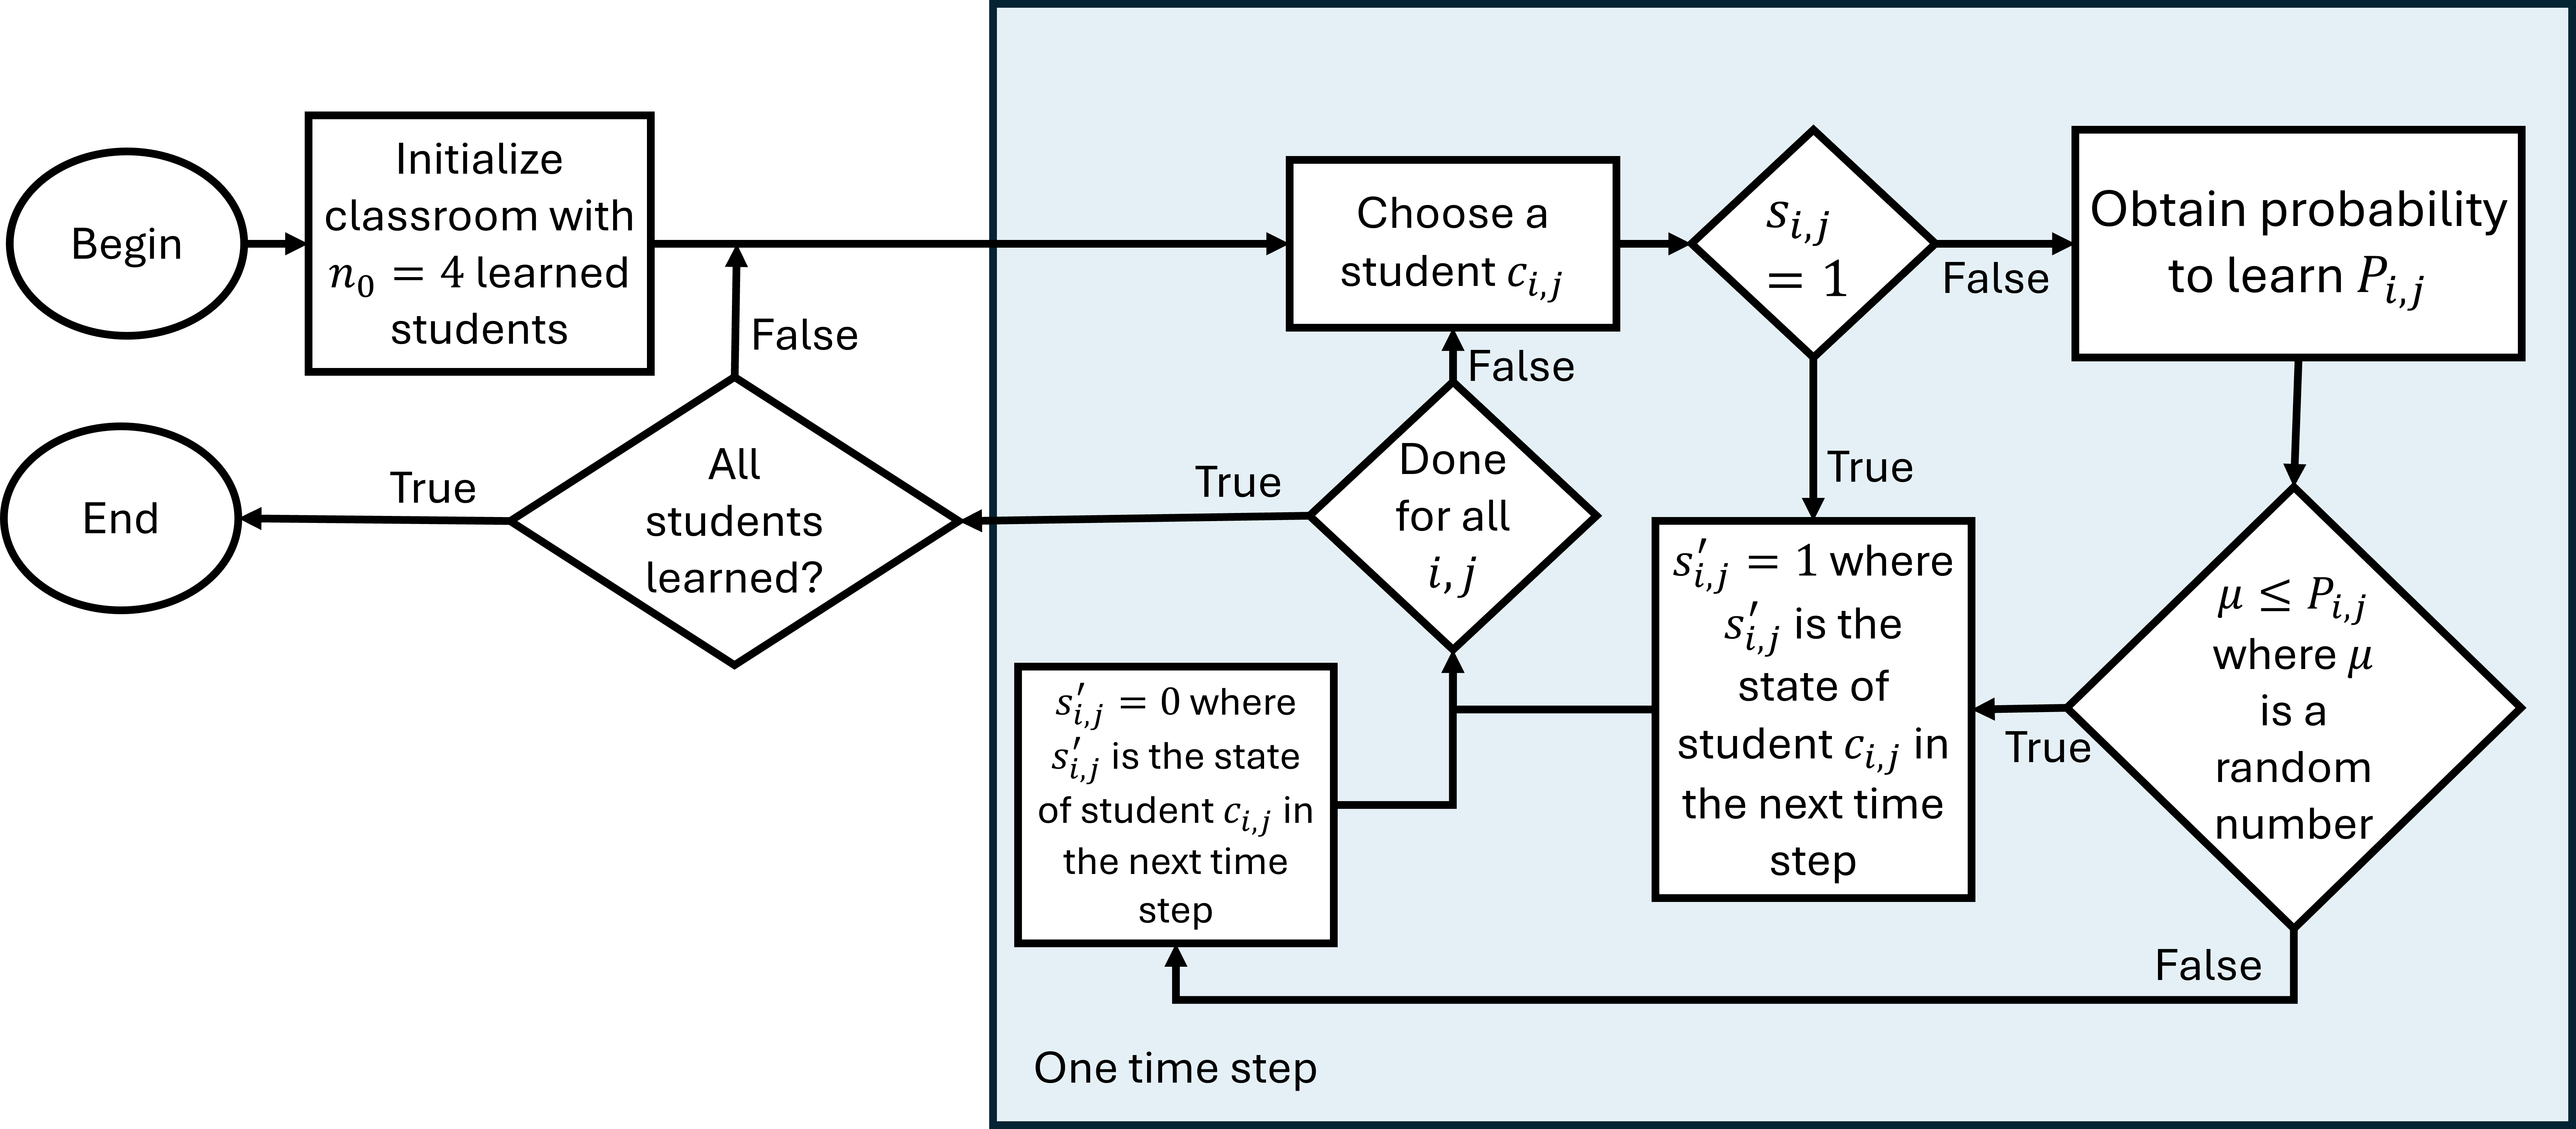
\includegraphics[width=\textwidth]{figs/2DBPCA Flowchart.png}
    \caption{
    Flowchart for the pCA algorithm used in this work.
    The broadcast (TI) and nearest-neighbor (PI) regimes differ in how the update probability $P_{i,j}$ is determined (Eqs.~\eqref{eq:TI-mode-probability} and~\eqref{eq:BPCA PI learning probability}, respectively).
    The next-step states $s'_{i,j}$ are applied to all agents together at the end of each time step (synchronous update), and the simulation ends once every agent has learned.
    }
    \label{fig:pCA-flowchart}
\end{figure}
The two regimes differ in how the update probability $P_{i,j}$ is determined, corresponding to the two modes of instruction being modeled.
These two interaction topologies are deliberately simplified representations of traditional and peer instruction, not complete descriptions of either pedagogy; the comparisons that follow therefore concern the relaxation dynamics of the model, not the educational effectiveness of the two instructional modes.

For the broadcast regime (traditional instruction, TI), the update probability is given by
%%
\begin{equation}
\label{eq:TI-mode-probability}
    P_{i,j} = \lambda_{i,j}\;\rho_{\delta i,\delta j}
\end{equation}
%%
where $\rho_{\delta i,\delta j}\in[0,1]$ encodes the potential dependence of the learning efficiency on the relative position of the information source with respect to the agent~\citep{dong2021influence}.
In the broadcast regime, each agent receives information directly from a global source, analogous to a lecturer addressing the entire class simultaneously.
We simplify by fixing $\rho_{\delta i,\delta j}=\rho_0$ as a uniform, isotropic coupling strength, giving $P_{i,j}=\lambda_{i,j}\rho_0$.

For the nearest-neighbor regime (peer instruction, PI), the update probability additionally depends on the states of adjacent agents.
The compounded probability of learning from any learned neighbor is given by
%%
\begin{equation}
\label{eq:BPCA PI learning probability}
    P_{i,j} = 1 - \prod_{\forall \delta i, \delta j}{\left[1-(\lambda_{i,j}\;\rho_{\delta i, \delta j})(s_{i+\delta i, j+\delta j})\right]}
\end{equation}
%%
where the product runs over all neighbors of agent $(i,j)$, and $s_{i',j'}$ is the state of the neighboring agent at position $(i'=i+\delta i,\; j'=j+\delta j)$.
We again simplify by fixing $\rho_{\delta i,\delta j}=\rho_0$ for $|\delta i|\leq1$ and $|\delta j|\leq1$, and zero otherwise, corresponding to a Moore neighborhood with isotropic coupling~\citep{kari2005catheory, zaitsev2017generalized, louis2018probabilistic}.
Higher-order neighborhood interactions are possible but not considered here.

In both regimes, the update is stochastic: an unlearned agent at $(i,j)$ transitions to the learned state at time step $t$ if and only if $u_{i,j}(t)\leq P_{i,j}$, where $u_{i,j}(t)\sim\mathcal{U}(0,1)$ is a random variate drawn from the continuous uniform distribution on $[0,1]$. An independent variate is drawn for every unlearned agent with a nonzero transition probability at every time step, so the $u_{i,j}(t)$ are independent and identically distributed across both agents and time. Learned agents are not updated (consistent with the absorbing-state assumption above) and are not assigned a variate.
The update is synchronous: the transition probabilities of all agents at time step $t$ are computed from the states at step $t-1$, and all resulting transitions are then applied simultaneously.
One time step is thus one learning step: the interval over which an unlearned agent learns with probability $\rho_0\lambda_{i,j}$ from the broadcast source, or from each learned neighbor. A time step therefore has no fixed duration in real time, such as a minute or a class session, and the model does not fix how many steps correspond to a given span of classroom time; Section~\ref{sec:rnd} shows that this choice does not affect the shape of the gain functions compared there (Eq.~\eqref{eq:k-step-gain}).

Simulations in both regimes are initialized with four learned agents placed according to the chosen seating arrangement, described below. Each broadcast run uses the same initially learned agents and the same assignment of learning rates as the nearest-neighbor run with the same parameters, so that paired runs of the two regimes differ only in the update rule.
The difference in update rule is the intended contrast between the two modes of instruction, and it differs in two ways: which agents are exposed, and how exposure accumulates.
In the broadcast regime every unlearned agent is exposed to the same source at every time step, with $P_{i,j}=\rho_0\lambda_{i,j}$.
In the nearest-neighbor regime only agents adjacent to learned agents are exposed, and exposure compounds over the $k$ learned neighbors as $P_{i,j}=1-(1-\rho_0\lambda_{i,j})^k$.
The two rules coincide for an agent with exactly one learned neighbor ($k=1$), so each learned neighbor acts as a source of the same strength as the broadcast source; the effects attributed to the interaction regime in Section~\ref{sec:rnd} arise from the restriction of exposure to the neighborhood of learned agents and from its compounding over neighbors.
Initially learned agents are required for the nearest-neighbor regime to evolve at all, and four is the smallest number that seeds each seating arrangement symmetrically: one agent per anchor point for the corner arrangements (Table~\ref{tbl:SA-rules}), and, for even $L$, the $2\times2$ block of sites surrounding the lattice center for the center arrangement.
These four agents, $4/N\leq0.4\%$ of the population, have a negligible effect in the broadcast regime, where they do not influence other agents.

The total relaxation time $t_{\rm max}$ is defined as the number of iterations until every agent has transitioned to the learned state, i.e.\ until the system reaches its absorbing state.
We also record $t_{95}$, the first iteration at which at least $95\%$ of agents have learned, which measures how quickly most of the population learns, independently of the last few agents.
Since the lattice is connected and every unlearned agent with at least one learned neighbor (nearest-neighbor regime), or every unlearned agent (broadcast regime), has a nonzero transition probability, the fully learned state is reached with probability one in both regimes.
Because learned agents are never updated, the cost of a time step scales with the number of agents that remain unlearned, so even runs with very slow residual learners remain inexpensive; for example, at $\rho_0=0.1$ and $\delta\lambda=0.49$ the low-$\lambda$ agents transition with probability $\rho_0(\lambda_0-\delta\lambda)=10^{-3}$ per step.
A safety cap of $10^{6}$ iterations was imposed but never reached: all $100{,}800$ simulation runs reported in this work reached the fully learned state.

The spatial configuration of initially learned agents in the nearest-neighbor regime is determined by the seating arrangement (SA), illustrated in Fig.~\ref{fig:PI-SAs}.
\begin{figure}[htbp]
    \centering
    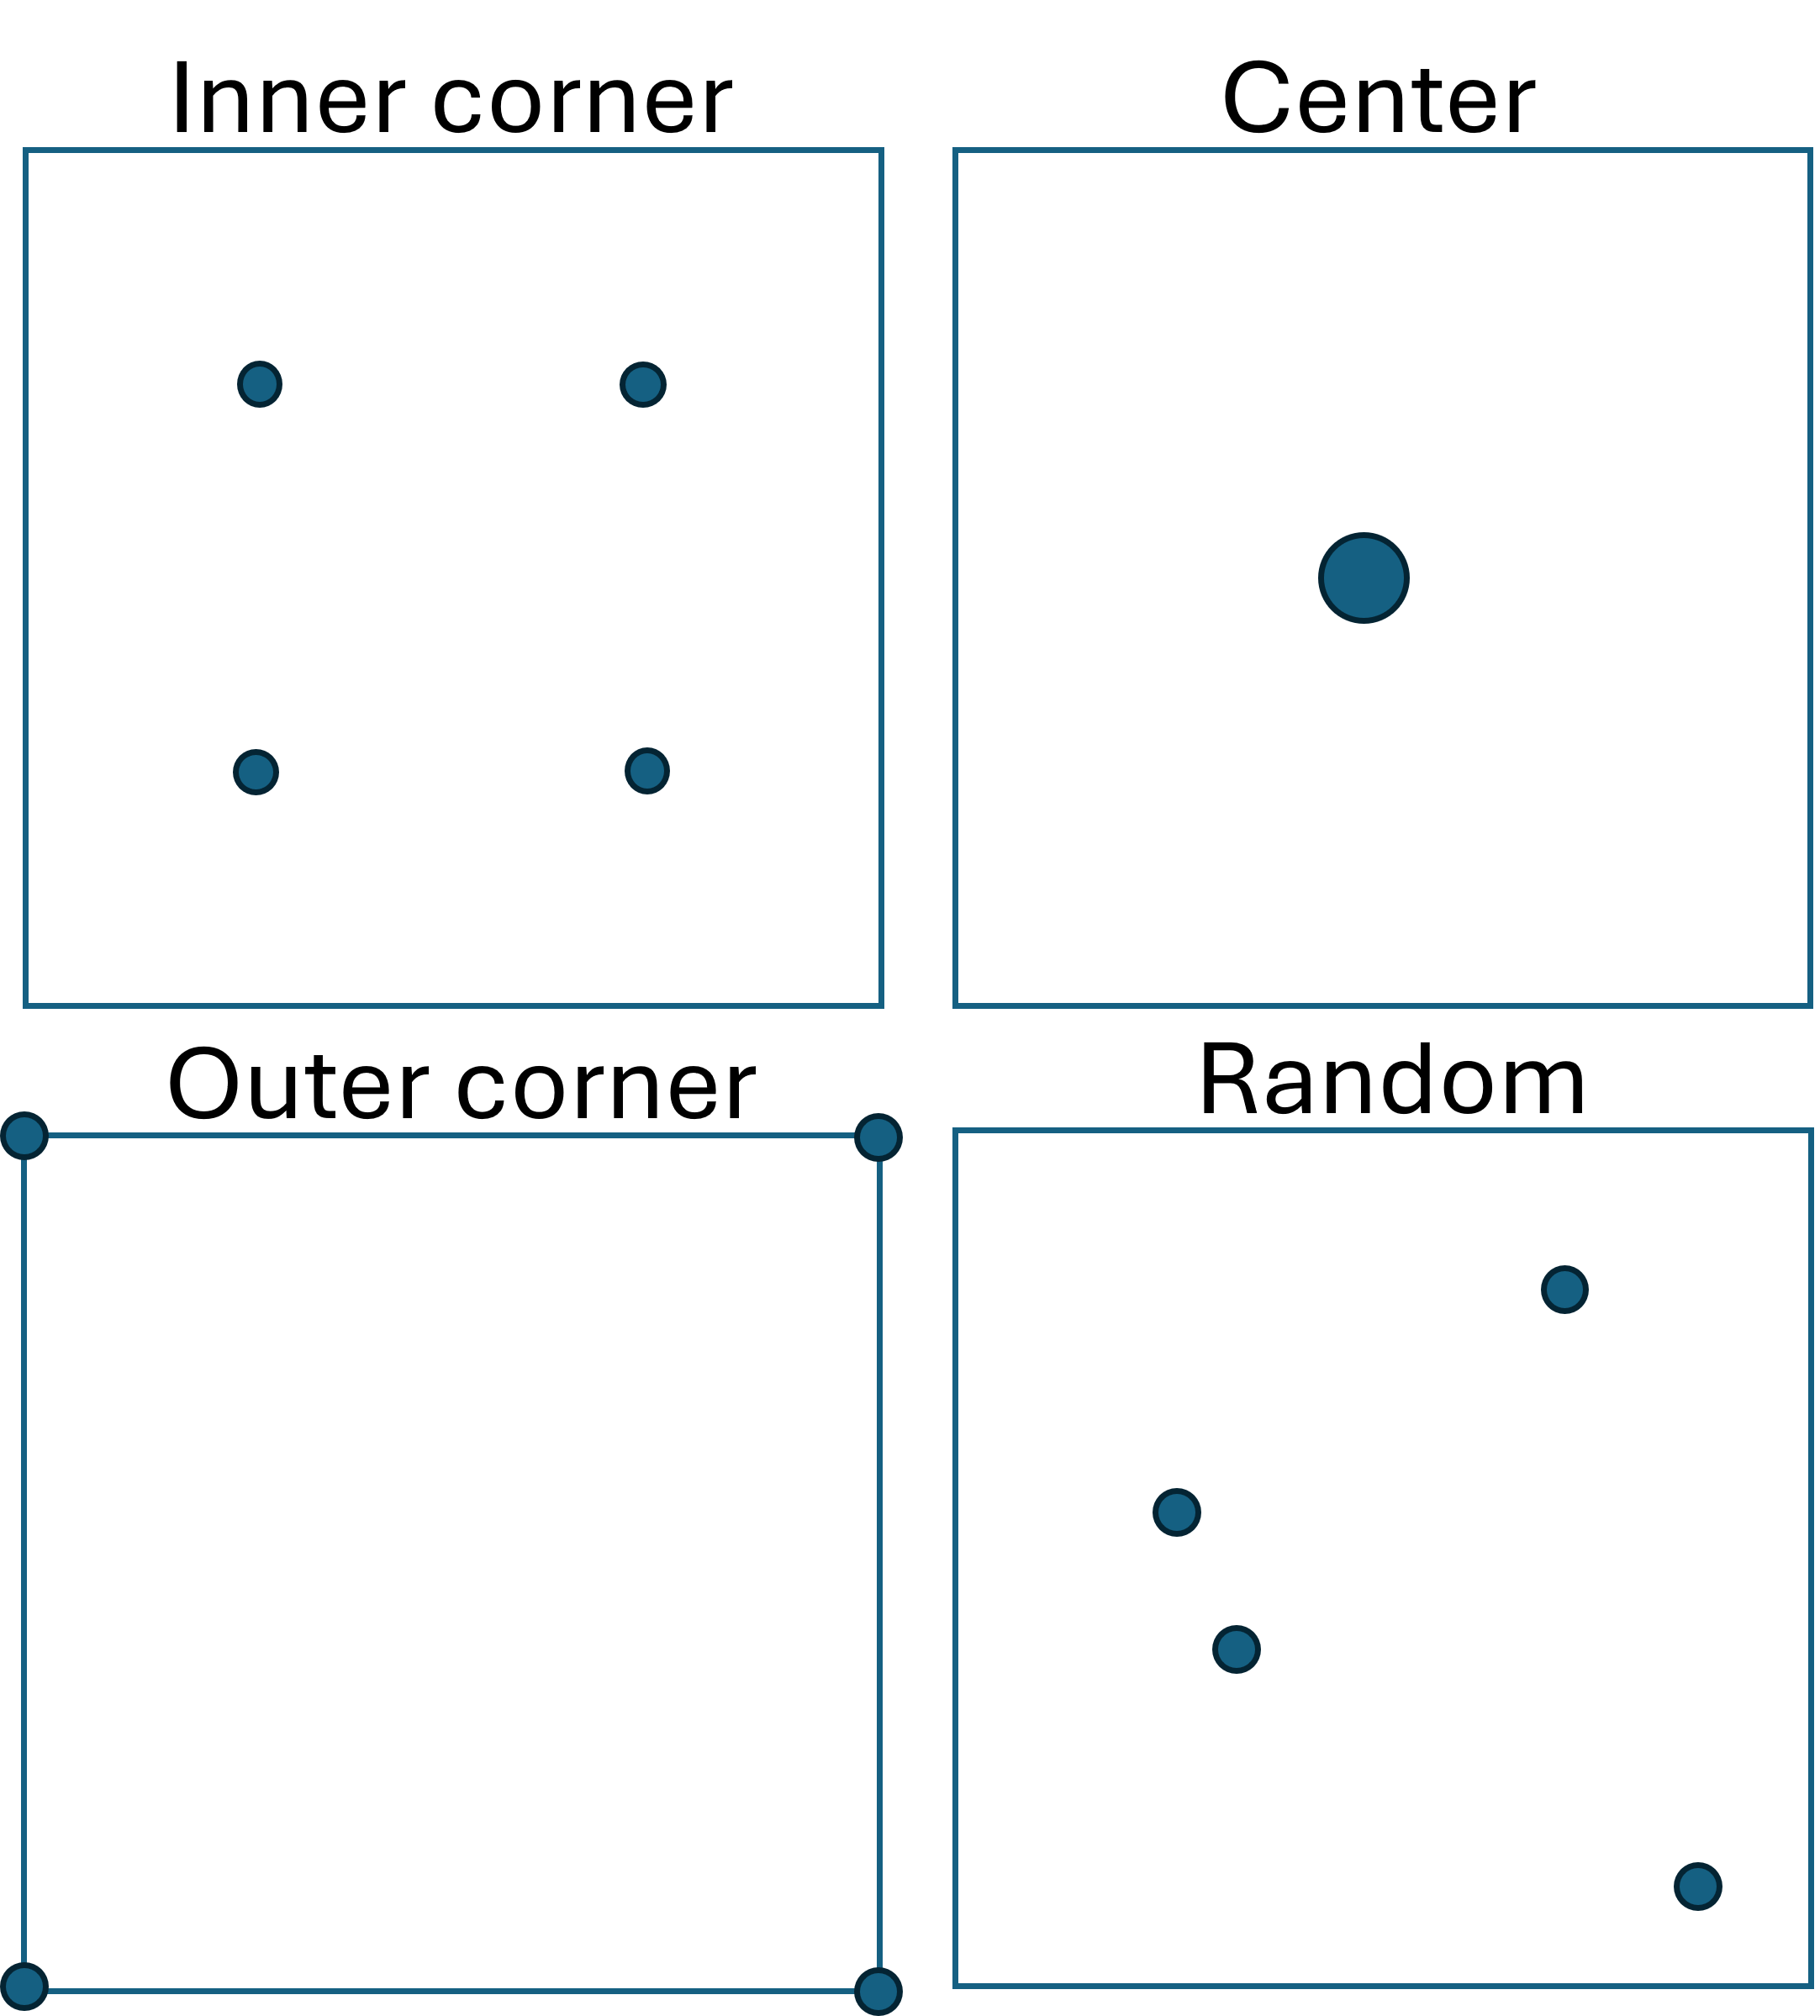
\includegraphics[width=0.50\textwidth]{figs/PI SAs.png}
    \caption{
    Seating arrangements (SAs) considered for the nearest-neighbor (PI) regime.
    Dots represent the initial positions of learned agents ($s_{i,j}=1$) in the lattice.
    Agents are otherwise arranged in a rectangular lattice pattern (shown here as square for brevity).
    The random case shown is one of many possible arrangements.
    }
    \label{fig:PI-SAs}
\end{figure}
Four arrangements are considered: inner corner, outer corner, center, and random, following prior work on the role of seating in classroom learning~\citep{roxas2010seating, monterola2009}.
For the first three, the initially learned agents occupy the lattice sites closest, in Euclidean distance, to the anchor points listed in Table~\ref{tbl:SA-rules}, with ties broken at random; for the random arrangement, the sites are drawn uniformly without replacement.
Unless otherwise specified, the inner corner arrangement is used as the default for the nearest-neighbor regime in the results that follow.
\begin{table}[htbp]
\caption{Placement of the initially learned agents for each seating arrangement on an $L\times L$ lattice with sites $(i,j)$, $i,j\in[1,L]$. Initially learned agents occupy the sites closest to the anchor points (Euclidean distance, ties broken at random); $q=L/4$.}
\label{tbl:SA-rules}
\begin{tabular*}{\tblwidth}{@{}l@{\extracolsep{\fill}}ll@{}}
\toprule
Arrangement & Anchor points & Initially learned sites (four agents) \\
\midrule
Outer corner & $(1,1)$, $(1,L)$, $(L,1)$, $(L,L)$ & The four corner sites \\
Inner corner & $(q,q)$, $(q,L-q+1)$, $(L-q+1,q)$, $(L-q+1,L-q+1)$ & The four anchor sites \\
Center & $\left(\tfrac{L+1}{2},\tfrac{L+1}{2}\right)$ & The central $2\times2$ block \\
Random & None & Drawn uniformly without replacement \\
\bottomrule
\end{tabular*}
\end{table}

For each regime and seating arrangement, we simulate every combination of $L\in\{32,48,64,96,128\}$, $\rho_0\in\{0.1,0.2,\dots,1.0\}$, and the seven values of $\delta\lambda$ above, with 20 independent runs per combination.
Each run uses its own pseudorandom number stream, initialized from a recorded seed, so that every run can be reproduced exactly.
With four initially learned agents on every lattice, a larger lattice also has a smaller initial learned fraction and a larger distance to the nearest learned agent.
To separate these effects from system size, we repeat the sweep for $L\geq48$ with the initial learned fraction fixed at that of the $L=32$ lattice, i.e.\ with $4L^2/32^2$ initially learned agents ($9$, $16$, $36$, and $64$), placed by the same rule (Table~\ref{tbl:SA-rules}).
Together, the two sets comprise $100{,}800$ runs.

\section{Results and Discussion}\label{sec:rnd}

The following results characterize the collective relaxation dynamics of the pCA model under both interaction regimes across a range of lattice side lengths $L$, coupling strengths $\rho_0$, and heterogeneity levels $\delta\lambda$.
All quantities presented are averages over twenty independent randomized runs. Bands show one standard deviation across runs, i.e.\ the spread of individual runs, whereas uncertainties of fitted coefficients are one standard error of the mean over runs; each caption states which is shown.

\subsection{Relaxation dynamics: broadcast versus nearest-neighbor regimes}

  The two regimes exhibit qualitatively distinct relaxation dynamics, as shown in Fig.~\ref{fig:comparison size}.
  In the broadcast regime, the global coupling mechanism drives a rapid early onset of transitions across the entire agent population simultaneously, with the relaxation rate tapering off in the later stages as agents with lower $\lambda$ values transition more slowly.
  In the nearest-neighbor regime, the spread of the learned state is governed by local propagation: learning spreads outward from the initially learned agents through contact between neighbors, as a connected front, producing a gradual initial increase in the learned fraction followed by a sharp rise as the number of active learned-unlearned interfaces grows.
  The nearest-neighbor regime catches up to and surpasses the broadcast regime in the later stages of relaxation, particularly for smaller lattice side lengths, and this observation holds consistently across all seating arrangements considered.
  This two-stage relaxation behavior, an early broadcast-driven stage followed by a surge driven by local propagation, becomes particularly pronounced under high heterogeneity, as discussed in the following subsection.

  \begin{figure}[htbp]
    \centering
    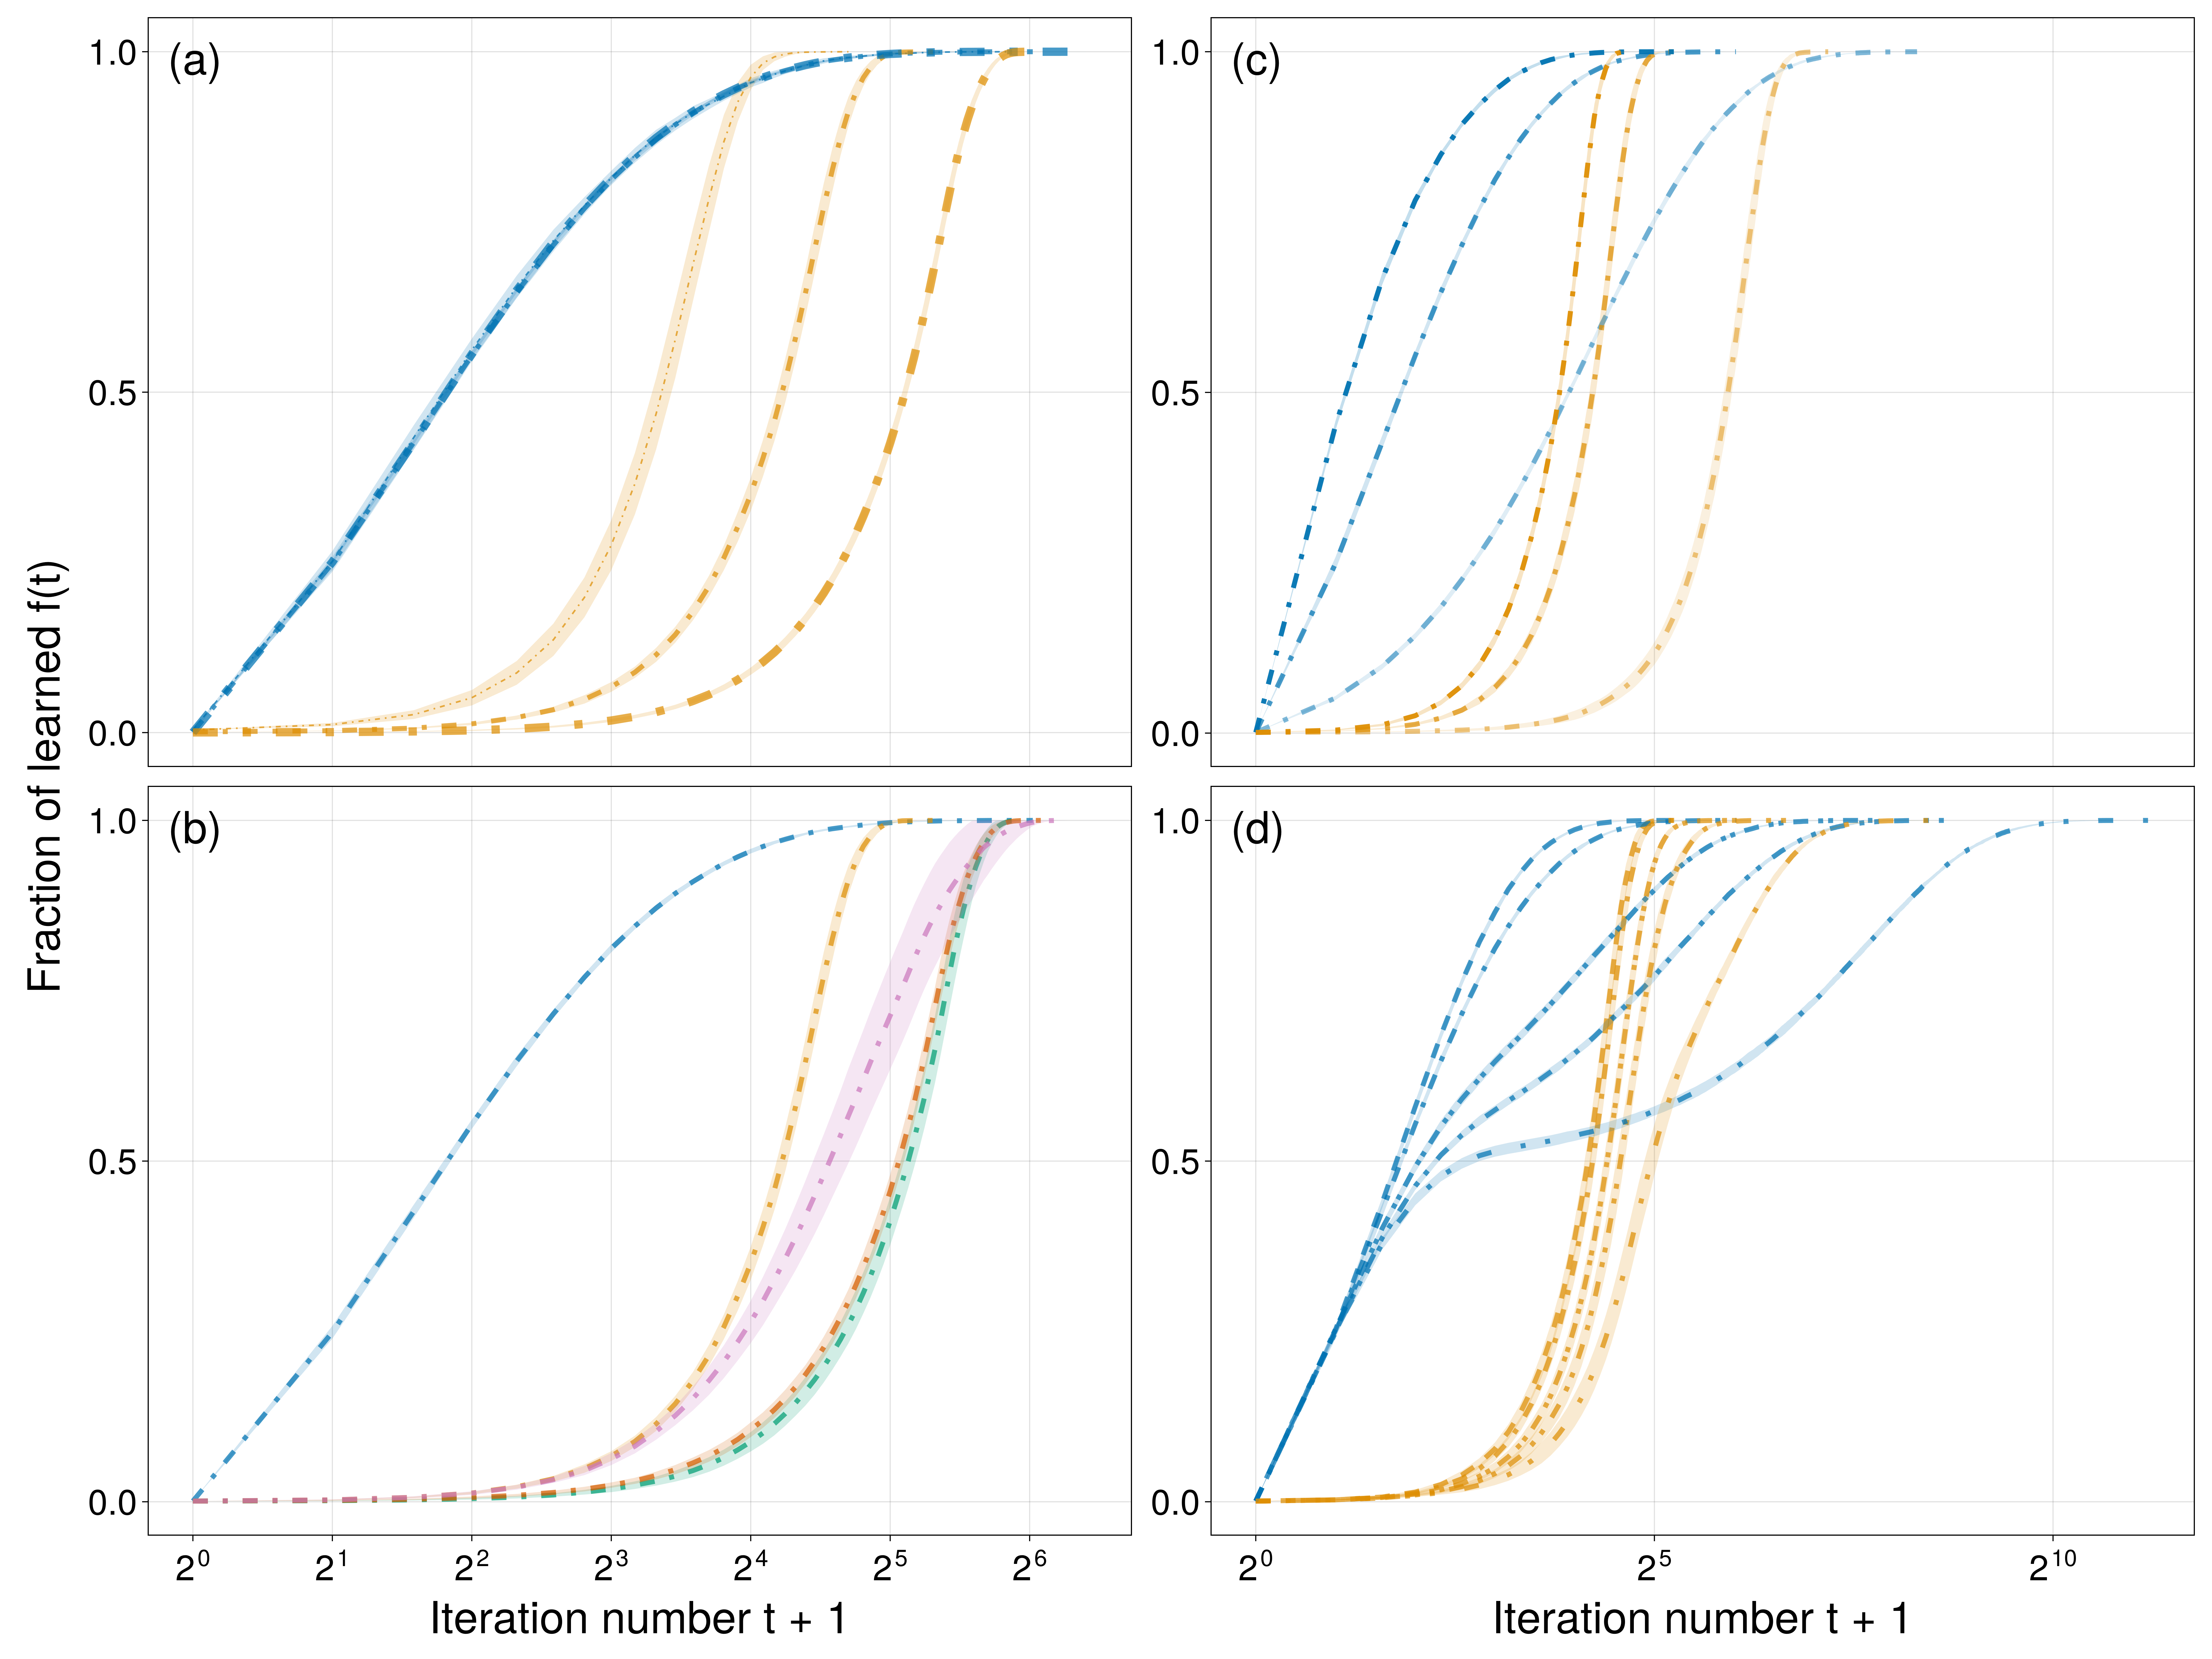
\includegraphics[width=0.8\textwidth]{figs/figure3-v2.png}
    \caption{
    Monotonic increase of the learned agent fraction over iteration number for both interaction regimes.
    The horizontal axis (iteration number) is shown on a base-2 logarithmic scale ($2^0, 2^1, 2^2, \dots$).
    Blue corresponds to the broadcast (TI) regime; all other colors correspond to the nearest-neighbor (PI) regime.
    Bands represent one standard deviation across $20$ independent randomized runs.
    (a)~Effect of lattice side length $L$ (line width proportional to lattice side length $L$); the inner corner SA is used for the nearest-neighbor regime; $\rho_0=0.5$, $\delta\lambda=0.2$.
    (b)~Effect of seating arrangement (SA) for a fixed lattice side length; colors indicate different SAs (yellow-orange: inner corner, orange: center, green: outer corner, pink: random); $\rho_0=0.5$, $\delta\lambda=0.2$.
    (c)~Effect of coupling strength $\rho_0$; inner corner SA, $L=64$, $\delta\lambda=0.2$.
    (d)~Effect of heterogeneity parameter $\delta\lambda$; inner corner SA, $L=64$, $\rho_0=0.5$.
    }
    \label{fig:comparison size}
  \end{figure}

  Fig.~\ref{fig:comparison size}(a) shows the effect of lattice side length $L$ on the relaxation curves.
  Note that the iteration axis in Fig.~\ref{fig:comparison size} is logarithmic (base~2): the log scale stretches out the early iterations relative to a linear axis, making the early transitions appear more gradual than they are, while compressing the already comparatively flat long tail of the later stage driven by local propagation into a narrow band, so the visual prominence of each stage should be read with the scale in mind.
  The broadcast regime is largely unaffected by lattice side length, as expected from the global coupling mechanism in which each agent updates independently of its neighbors.
  In the nearest-neighbor regime, increasing $L$ delays the onset of the sharp rise in the learned fraction without significantly affecting the slope of that rise, resulting in a shift of $t_{\rm max}$ with lattice side length while the overall curve shape is preserved.
  Part of this shift could reflect the smaller initial learned fraction on larger lattices rather than system size itself.
  We quantify the size dependence by the scaling exponent $\gamma$ of $t_{\rm max}\propto L^{\gamma}$, obtained as the slope of $\log t_{\rm max}$ against $\log L$ from $L=32$ to $L=128$; $\gamma$ would be $1$ for a front advancing at constant speed across the lattice and $0$ for no size dependence.
  Holding the initial learned fraction fixed (Appendix~\ref{app:seed density}) leaves the size dependence of the clustered arrangements essentially unchanged: at $\rho_0=0.5$ and $\delta\lambda=0.2$, $\gamma$ is $0.81$ with four initially learned agents and $0.78$ with a fixed fraction for the inner corner arrangement, and similarly for the center ($0.91$ and $0.89$) and outer corner ($0.93$ and $0.89$) arrangements, and the two exponents remain close across all $\rho_0$ and $\delta\lambda$.
  For clustered initial conditions, the learned front must cross a distance proportional to $L$, so the size dependence is intrinsic to nearest-neighbor propagation.
  For the random arrangement, by contrast, $\gamma$ falls from $0.91$ to $0.18$: there, the size dependence comes mostly from the dilution of the initially learned agents.

  Fig.~\ref{fig:comparison size}(b) shows the effect of seating arrangement on the nearest-neighbor regime.
  The inner corner arrangement produces the earliest onset of the sharp rise, outperforming all other arrangements considered.
  Similarly to the effect of system size, different seating arrangements primarily shift the onset of the sharp rise rather than its slope, with the exception of the random arrangement, which affects both the slope of the rise and exhibits the widest spread across runs.
  The center and outer corner arrangements perform similarly, a consequence of the isotropic coupling assumption in the model.

\subsection{Effects of coupling strength and agent heterogeneity}\label{sec:heterogeneity}

    The coupling strength $\rho_0$ and heterogeneity parameter $\delta\lambda$ are the two key parameters governing the relaxation dynamics, and their effects are shown in Fig.~\ref{fig:comparison size}(c,d).

    As shown in Fig.~\ref{fig:comparison size}(c), increasing $\rho_0$ shifts the relaxation curve earlier along the iteration axis for both regimes, reflecting the higher per-step probability of transitioning to the learned state.
    This shift is nonlinear: a change from $\rho_0=0.1$ to $0.5$ produces a larger shift than the same increment from $\rho_0=0.5$ to $0.9$.
    The broadcast regime shows an earlier onset of learning for all values of $\rho_0$, consistent with its global coupling mechanism.
    The nearest-neighbor regime, by contrast, exhibits a more stable curve shape across varying $\rho_0$, with coupling strength introducing primarily a delay in onset rather than a change in the character of the relaxation.

    The effect of agent heterogeneity $\delta\lambda$ is shown in Fig.~\ref{fig:comparison size}(d) and reveals a qualitative difference between the two regimes.
    In the broadcast regime, increasing $\delta\lambda$ introduces a pronounced two-stage relaxation: a fast initial stage driven by the high-$\lambda$ subpopulation, followed by a slow residual stage as the low-$\lambda$ subpopulation transitions on a longer timescale.
    This two-stage behavior becomes most pronounced at $\delta\lambda=0.45$, where the separation between the two relaxation stages is most clearly visible.
    At the extreme value of $\delta\lambda=0.49$ (subpopulations with $\lambda=0.01$ and $\lambda=0.99$), the two stages are separated by roughly two orders of magnitude in time.
    On the logarithmic iteration axis of Fig.~\ref{fig:comparison size}(d), the curve rises as the high-$\lambda$ subpopulation learns, plateaus near $f=1/2$, rises again as the low-$\lambda$ subpopulation transitions, and finally saturates.
    This alternation of fast and slow stages is the two-rate relaxation described above rather than a distinct mechanism.
    Because agents in the broadcast regime transition independently of one another, the expected learned fraction (excluding the initially learned agents) is exactly
    $F(t)=1-w(1-p_+)^t-(1-w)(1-p_-)^t$, with $p_\pm=\rho_0(\lambda_0\pm\delta\lambda)$ and $w\approx1/2$ the fraction of high-$\lambda$ agents, and the mean of the simulated runs agrees with $F(t)$ to within $1.5\times10^{-3}$ at every time step.

    In the nearest-neighbor regime, heterogeneity produces only a gradual delay in the relaxation curve across all values of $\delta\lambda$ considered, with no qualitative change in curve shape apart from a slower final approach to $f=1$ at $\delta\lambda\geq0.45$, where the last low-$\lambda$ agents take longer to learn: the local propagation process effectively averages over the heterogeneous $\lambda$ distribution as the learned state propagates through the lattice.
    Following the high- and low-$\lambda$ agents separately (Fig.~\ref{fig:class split}) shows why.
    In the broadcast regime the two subpopulations learn on separate timescales, and the curve of the whole population lies between the two, whereas in the nearest-neighbor regime a low-$\lambda$ agent is usually reached by the front only after several of its neighbors have learned, which multiplies its transition probability (Eq.~\eqref{eq:BPCA PI learning probability}).
    For $L=128$, the time for half of the low-$\lambda$ agents to learn exceeds that for half of the high-$\lambda$ agents by at most $13\%$ in the nearest-neighbor regime for $\delta\lambda\leq0.4$, compared with a factor of up to $8$ in the broadcast regime; at $\delta\lambda=0.49$ the factors are about $2$ and $45$--$90$, respectively.

    \begin{figure}[htbp]
        \centering
        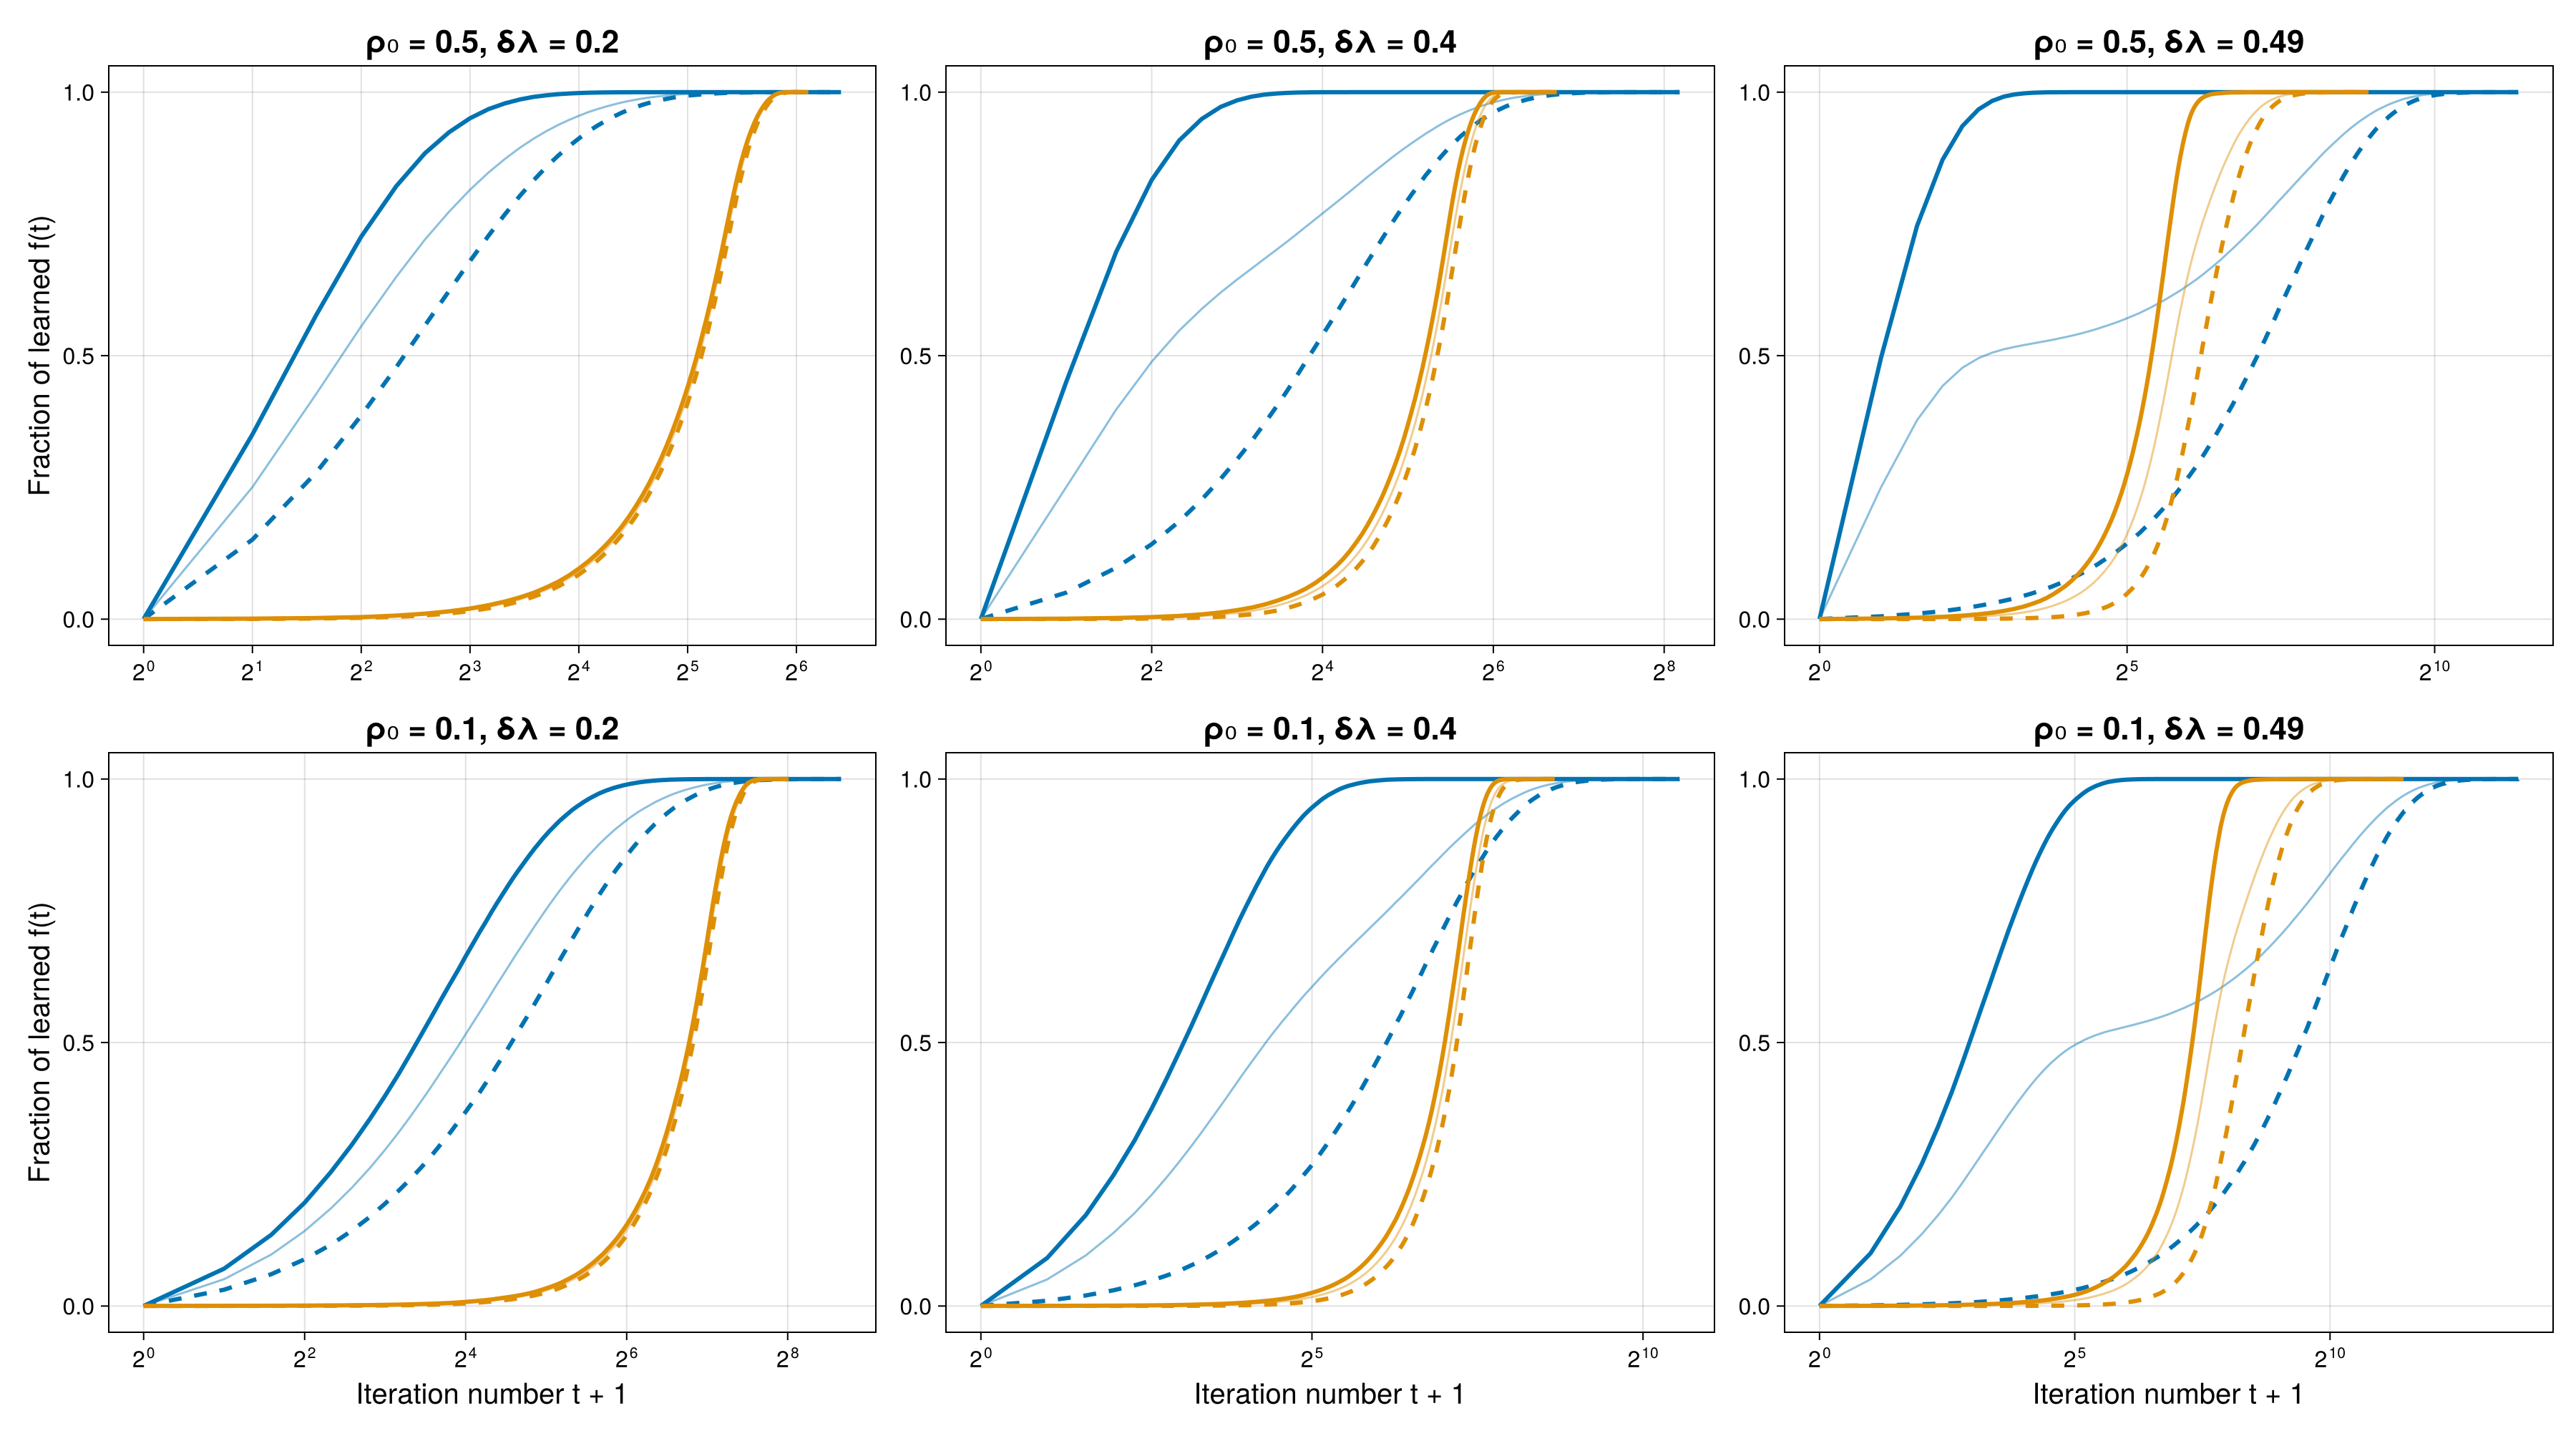
\includegraphics[width=\textwidth]{figs/figure-class-split.png}
        \caption{Fraction of learned agents among the high-$\lambda$ agents (thick solid lines) and the low-$\lambda$ agents (thick dashed lines), and in the whole population (thin lines), for the broadcast (blue) and nearest-neighbor (orange, inner corner arrangement) regimes, with $L=128$, $\rho_0=0.5$ (top row) and $\rho_0=0.1$ (bottom row), and $\delta\lambda=0.2$, $0.4$, and $0.49$ (left to right); means over 20 runs. The iteration axis is logarithmic (base~2).}
        \label{fig:class split}
    \end{figure}

    The spatial evolution of the learned state across the lattice provides further insight into these dynamical differences, as shown in Fig.~\ref{fig:spatial config} for a smaller lattice side length $L=32$ for visual clarity.
    In the broadcast regime, agents with high $\lambda$ values transition first, appearing as isolated learned sites distributed across the lattice, with low-$\lambda$ agents filling in slowly afterward.
    In the nearest-neighbor regime, the learned state spreads outward from the initial seed sites as a connected front, with this local propagation producing the characteristic sharp rise in the learned fraction observed in the relaxation curves.
    These observations suggest a hypothesis: a combination of both regimes, with an initial broadcast phase that seeds learned agents throughout the lattice followed by a nearest-neighbor phase that propagates learning from those sites, could combine the rapid, population-wide onset of the broadcast regime with the front-like spreading of the nearest-neighbor regime, which leaves no isolated unlearned agents behind. Such a sequence parallels current instructional practice~\citep{mazur1997peer, smith2009peer, lasry2008peer, roxas2010seating}, but the present model simulates each regime separately, so this hypothesis is not tested here.

    \begin{figure}[htbp]
        \centering
        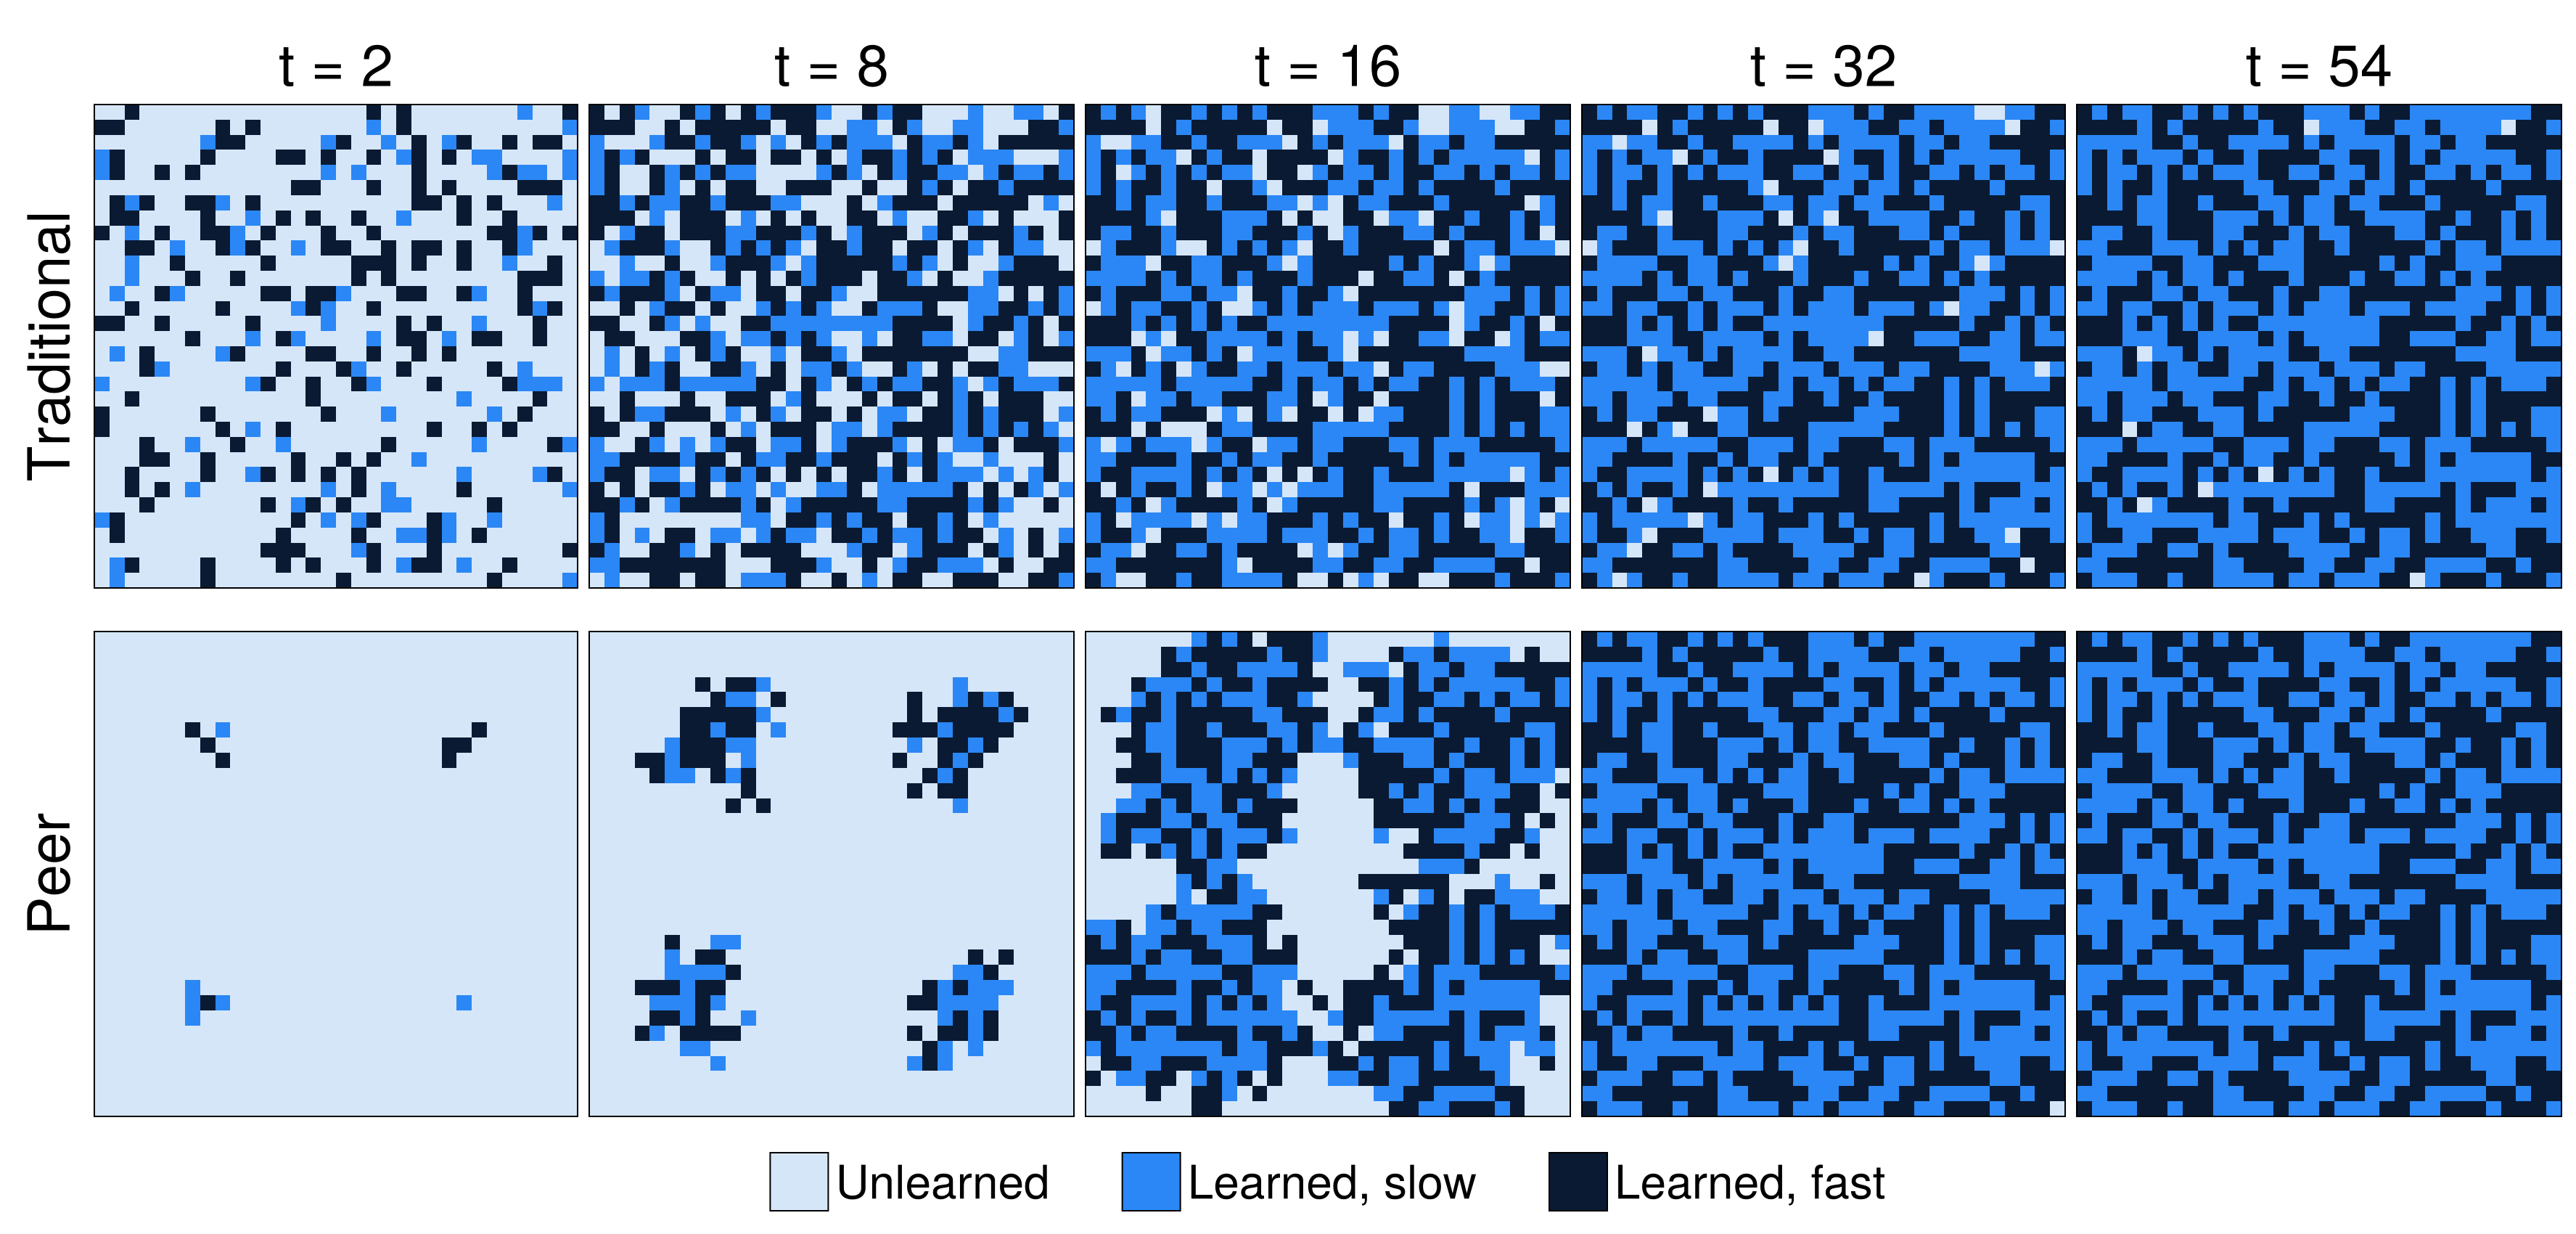
\includegraphics[width=0.9\textwidth]{figs/figure4-v2.png}
        \caption{
        Representative spatial configurations of the lattice ($L=32$, $\rho_0=0.3$, $\delta\lambda=0.2$) at iteration numbers $t=2,8,16,32$, and $54$, for the broadcast (top row, ``Traditional'') and nearest-neighbor (bottom row, ``Peer'') regimes, from one pair of runs with the same four initially learned agents (inner corner arrangement) and the same assignment of learning rates.
        Light blue indicates unlearned agents; blue and dark navy indicate learned agents with slow and fast learning rates $\lambda$, respectively.
        }
        \label{fig:spatial config}
    \end{figure}

\subsection{Combined effects of coupling strength and heterogeneity}

    The combined effects of coupling strength $\rho_0$ and heterogeneity $\delta\lambda$ on the total relaxation time $t_{\rm max}$ are summarized in Fig.~\ref{fig:Params effect summary t} for two lattice side lengths, $L=32$ and $L=128$ (populations $N=1024$ and $N=16384$).
    Higher $t_{\rm max}$ is disadvantageous, corresponding to slower collective relaxation of the agent population.

    For small lattice side lengths (Fig.~\ref{fig:Params effect summary t}(a)), the nearest-neighbor regime has the shorter $t_{\rm max}$ for all but the lowest heterogeneity, and the difference grows with $\delta\lambda$.
    This advantage diminishes at higher coupling strength $\rho_0$, where the broadcast regime benefits more strongly from increased coupling strength.
    For large lattice side lengths (Fig.~\ref{fig:Params effect summary t}(b)), this relationship reverses at low heterogeneity: the broadcast regime has the shorter $t_{\rm max}$ for every $\rho_0$ at $\delta\lambda=0$ and for most $\rho_0$ up to $\delta\lambda=0.2$.

    In absolute terms the difference is asymmetric: over the range of Fig.~\ref{fig:Params effect summary t}, the broadcast regime is faster by at most $27$ iterations, whereas the nearest-neighbor regime can be faster by more than $600$ iterations at high heterogeneity.
    As ratios, however, the two are comparable: the nearest-neighbor regime is at most $2.8$ times slower than the broadcast regime, and the broadcast regime at most $3.9$ times slower than the nearest-neighbor regime.

    Which regime relaxes faster also depends on how relaxation is measured (Fig.~\ref{fig:Params effect summary t}(c,d); Appendix~\ref{app:t95} shows both measures over the full range of heterogeneity, with their run-to-run spread).
    In the broadcast regime, agents transition independently, so for a homogeneous population with per-step transition probability $p$ the unlearned fraction after $t$ steps is $(1-p)^t$. Setting this fraction to $1/20$ ($95\%$ learned) gives $t_{95}$, and setting it to $1/N$ (a single agent left unlearned) gives $t_{\rm max}$:
    %%
    \begin{equation}
        t_{95}\approx\frac{\ln 20}{|\ln(1-p)|}, \qquad
        t_{\rm max}\approx\frac{\ln N}{|\ln(1-p)|}, \qquad
        \frac{t_{95}}{t_{\rm max}}\approx\frac{\ln 20}{\ln N}.
    \label{eq:tmax-t95}
    \end{equation}
    %%
    Thus $t_{95}$ does not depend on the population size, whereas $t_{\rm max}$, the time of the last of $N$ agents, grows as $\ln N$.
    The ratio $t_{95}/t_{\rm max}$ is the fraction of the total relaxation time needed for $95\%$ of agents to learn; its predicted value agrees with the simulated broadcast runs at $\delta\lambda=0$ (Table~\ref{tbl:tmax-t95}), and heterogeneity lowers it further, since the last agent to learn is then also a low-$\lambda$ agent.
    In the broadcast regime, $95\%$ of agents have therefore learned within the first $25$--$42\%$ of the total relaxation time, and the remainder is spent on the last few agents.
    In the nearest-neighbor regime, the learned front reaches agents in order of their distance from the initially learned agents, so few are left behind and $95\%$ learned is reached only at $57$--$81\%$ of the total relaxation time.
    As a result, for $L=128$ the broadcast regime reaches $95\%$ learned sooner for every $\rho_0$ up to $\delta\lambda=0.3$, even where its $t_{\rm max}$ is the longer of the two.
    For example, at $\rho_0=0.5$ and $\delta\lambda=0.3$, the last agent learns after $95$ iterations in the broadcast regime and after $68$ in the nearest-neighbor regime, yet $95\%$ of agents have learned after only $22$ iterations in the broadcast regime, compared with $51$ in the nearest-neighbor regime.
    The nearest-neighbor regime has the shorter $t_{95}$ only at high heterogeneity or for $L=32$.
    Within the model, the broadcast regime thus brings most of the population to the learned state quickly, while the nearest-neighbor regime is better at ensuring that no agent is left far behind.
    This complementarity, the broadcast regime bringing most agents to the learned state quickly and the nearest-neighbor regime leaving few agents behind and remaining robust under heterogeneity, motivates the hypothesis that a combination of both regimes could outperform either one alone. Whether, and under which conditions, such a combination is optimal requires simulating the combined regime directly, which we leave to future work.

    \begin{figure}[htbp]
        \centering
        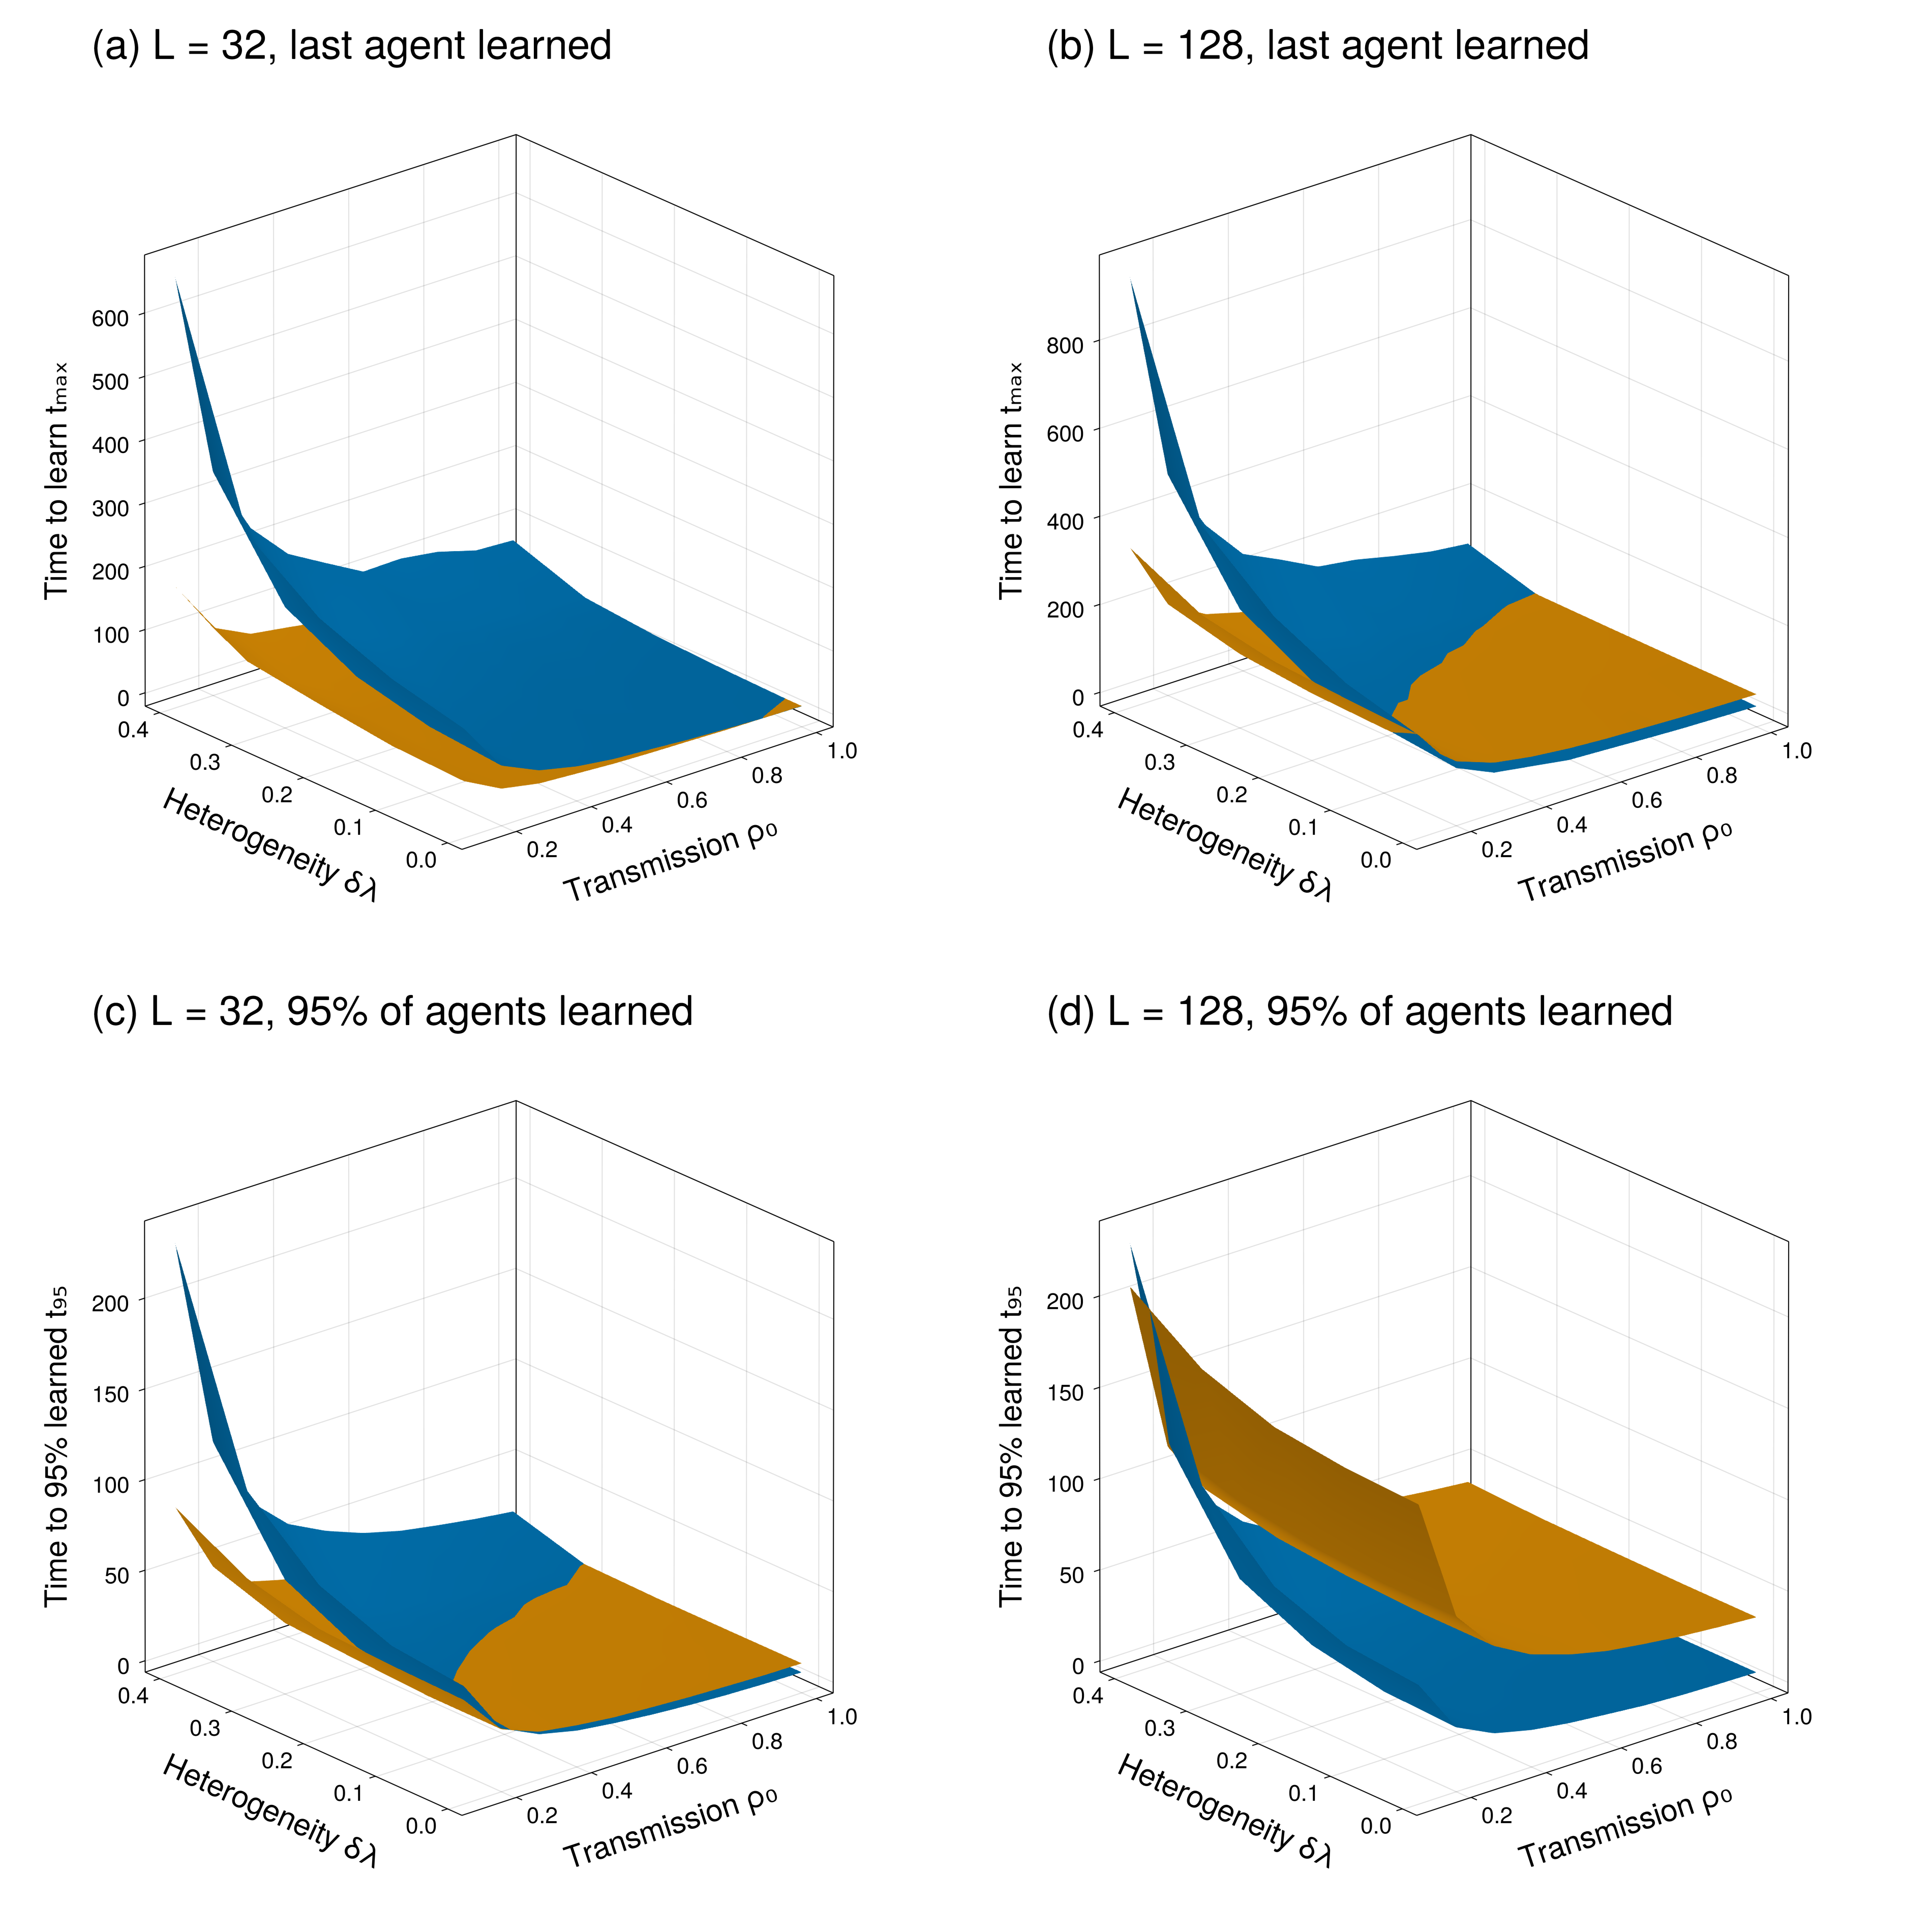
\includegraphics[width=0.8\textwidth]{figs/figure5-v2.png}
        \caption{
        Total relaxation time $t_{\rm max}$ (top row, last agent learned) and time $t_{95}$ for $95\%$ of agents to learn (bottom row) as functions of coupling strength $\rho_0$ and heterogeneity $\delta\lambda$, for the broadcast (blue surface) and nearest-neighbor (orange surface) regimes, for lattice side lengths $L=32$ (a,~c) and $L=128$ (b,~d); means over 20 runs.
        The nearest-neighbor regime uses the inner corner seating arrangement.
        Lower values indicate faster collective relaxation.
        }
        \label{fig:Params effect summary t}
    \end{figure}

    \begin{table}[htbp]
    \caption{Fraction of the total relaxation time needed for $95\%$ of agents to learn, $t_{95}/t_{\rm max}$, for the inner corner arrangement. Each entry averages this fraction over 20 runs at each of the ten coupling strengths $\rho_0=0.1,0.2,\dots,1.0$, since the predicted ratio does not depend on $\rho_0$ (the simulated broadcast values vary by at most $0.03$ across $\rho_0$). The prediction is Eq.~\eqref{eq:tmax-t95} for independently transitioning agents with $\delta\lambda=0$.}
    \label{tbl:tmax-t95}
    \begin{tabular*}{\tblwidth}{@{}l@{\extracolsep{\fill}}cccc@{}}
    \toprule
    & \multicolumn{2}{c}{$L=32$} & \multicolumn{2}{c}{$L=128$} \\
    & $\delta\lambda=0$ & $\delta\lambda=0.4$ & $\delta\lambda=0$ & $\delta\lambda=0.4$ \\
    \midrule
    Prediction, $\ln 20/\ln N$ & $0.43$ & -- & $0.31$ & -- \\
    Broadcast (TI) & $0.42$ & $0.35$ & $0.31$ & $0.25$ \\
    Nearest-neighbor (PI) & $0.79$ & $0.57$ & $0.81$ & $0.68$ \\
    \bottomrule
    \end{tabular*}
    \end{table}

\subsection{Comparison with empirical data and theoretical predictions}

    The return map, a plot of the learned fraction at iteration $t$ against that at iteration $t-1$, provides a means of characterizing the fixed-point structure of the relaxation dynamics and connecting simulation results to empirical classroom data.
    Following the mapping $S \rightarrow f$, where $f$ is the fraction of learned agents, the Hake gain $g$ can be approximated from simulation or empirical data via
    %%
    \begin{equation}\label{eq:gain-from-return-map}
    g(f) = \frac{h(f) - f}{1 - f}
    \end{equation}
    %%
    where $h(f)$ is a fitting function to the return map data following the recurrence relation $f_t = h(f_{t-1})$.

    Equation~\eqref{eq:gain-from-return-map} is singular at $f=1$, so the fitting function $h(f)$ must satisfy $h(1)=1$ for $g(f)$ to remain finite. For the simulation data this holds exactly: $f=1$ (all agents learned) is the absorbing state of the model, so $f_t=1$ maps to $f_{t+1}=1$ by construction. We therefore fit the simulation return maps with functional forms that impose $h(1)=1$ identically, which makes the singularity in Eq.~\eqref{eq:gain-from-return-map} removable: the limit as $f\to1$ is finite and recovers the gains reported below ($g=a_0$ for the broadcast regime; $g(1)=a_0-a_2$ for the nearest-neighbor regime). Consecutive points of one run are correlated, since each learned fraction is computed from the previous one, so a single fit to all points of all runs would understate the uncertainty of the coefficients. We therefore fit each of the 20 runs separately and report the mean of the coefficients over runs $\pm$ the standard error of the mean, treating the independent runs, rather than the points, as the samples. The empirical data are treated differently: real classes can exhibit score decreases from $f_{t-1}=1$ (a student answering correctly on the first assessment may answer incorrectly on the second), so there is no structural guarantee that $h(1)=1$. We therefore fit the empirical return map with a free (unconstrained) quadratic and do not evaluate the empirical gain at $f=1$.

    Fig.~\ref{fig:Return map} shows the return maps obtained from simulation data for both regimes across selected parameter sets, alongside empirical classroom data provided by Roxas \citep{monterola2009}.
    The broadcast regime consistently produces a linear return map, well described by
    %%
    \begin{equation}
        h(f) = a_0 + (1-a_0)f \;{\rm [broadcast]}
        \label{eq:ti-return-map}
    \end{equation}
    %%
    corresponding to a constant Hake gain $g(f) = a_0$ (fitted values in Table~\ref{tbl:returnmapfits}).
    For a homogeneous population ($\delta\lambda=0$) this form is exact: every unlearned agent transitions independently with probability $p=\rho_0\lambda_0$, so the unlearned fraction obeys $1-f(t+1)=(1-p)[1-f(t)]$, which gives $a_0=\rho_0\lambda_0$.
    For $\delta\lambda>0$, the high- and low-$\lambda$ agents transition with the fixed probabilities $p_\pm=\rho_0(\lambda_0\pm\delta\lambda)$, and the expected learned fraction $F(t)$ (Section~\ref{sec:heterogeneity}) gives the exact gain at step $t$,
    %%
    \begin{equation}
        g(t)=1-\frac{1-F(t+1)}{1-F(t)}=\frac{w p_+(1-p_+)^t+(1-w)p_-(1-p_-)^t}{w(1-p_+)^t+(1-w)(1-p_-)^t},
    \label{eq:ti-exact-gain}
    \end{equation}
    %%
    the mean of $p_\pm$ over the agents still unlearned.
    This gain starts at $\rho_0\lambda_0$ and decreases to $p_-$ as the high-$\lambda$ agents are depleted, so the fitted $a_0$ is an effective average over the relaxation.
    Its initial and final values differ by the factor $\lambda_0/(\lambda_0-\delta\lambda)$, independent of $\rho_0$.
    The per-step gain measured in the simulations agrees with Eq.~\eqref{eq:ti-exact-gain} to within $0.022\rho_0\lambda_0$ at every $f$ (Fig.~\ref{fig:ti gain}), and Table~\ref{tbl:ti gain} lists how far the fitted constant $a_0$ departs from it.
    The constant gain of Eq.~\eqref{eq:ti-return-map} is thus exact at $\delta\lambda=0$, a fair approximation for $\delta\lambda\leq0.2$, and only an effective average for stronger heterogeneity; the fitted $a_0$ varies by at most $3\%$ between $L=32$ and $L=128$.
    The nearest-neighbor return map, by contrast, is well described by a fitted quadratic
    %%
    \begin{equation}
        h(f) = a_0 + [1-(a_0+a_2)]f + a_2f^2 \;{\rm [nearest\text{-}neighbor]}
    \end{equation}
    %%
    corresponding to a linear Hake gain $g(f) = a_0 - a_2 f$, consistent with the theoretical prediction of~\citet{nitta2019mathematical} in the limit $a_0 \approx 0$ (fitted values in Table~\ref{tbl:returnmapfits}).
    Unlike the broadcast form at $\delta\lambda=0$, this quadratic is not derived from the update rule: in the nearest-neighbor regime the next learned fraction depends on the positions of the learned agents, not on $f$ alone, so no exact map for $f$ exists.
    The quadratic is therefore a fitted description of the simulated return maps over the parameter range of Fig.~\ref{fig:Return map} ($\delta\lambda\leq0.4$), used to summarize the shape of the gain.

    To separate the effect of system size from that of the other parameters, the panels in each row of Fig.~\ref{fig:Return map} share the same coupling strength and heterogeneity and differ only in $L$.
    The broadcast gain $a_0$ does not depend on $L$ (Table~\ref{tbl:returnmapfits}), as expected for agents that transition independently of one another.
    The nearest-neighbor coefficients, by contrast, decrease with $L$ at fixed $\rho_0$ and $\delta\lambda$.
    For every combination of $\rho_0\in\{0.1,0.5,0.9\}$ and $\delta\lambda\in\{0,0.2,0.4\}$, $|a_2|$ decreases as a power of the lattice side, $|a_2|\propto L^{-\beta}$ with $\beta$ between $0.5$ and $0.9$ over $L=32$ to $128$, with smaller $\beta$ at high heterogeneity and low coupling (Fig.~\ref{fig:coefs vs L}, Appendix~\ref{app:coefs vs L}).
    The exponents change by less than $0.01$ when the initial learned fraction, rather than the number of initially learned agents, is held fixed ($4L^2/32^2$ initially learned agents, the initial fraction of the $L=32$ lattice), so the decrease reflects the distance the learned state must cross rather than the dilution of the initial seeds.
    The magnitude $|a_2|$ therefore serves as a measure of the efficiency of the nearest-neighbor regime, which decreases with system size, consistent with the $t_{\rm max}$ results presented above.

    The empirical dataset, consisting of pre- and post-test scores from fourteen classrooms of 64 students each, spans a broad range of values and exhibits considerable scatter, reflecting the many factors influencing real classroom dynamics.
    A quadratic fit to this data yields a value of $a_2$ (Table~\ref{tbl:returnmapfits}), though the fit quality is limited by the variance in the data ($R^2=0.63$ over $N_{\rm pts}=896$ pre/post pairs, compared with $R^2>0.99$ for the simulation fits; Table~\ref{tbl:returnmapfits}).
    The sign of the empirical quadratic coefficient, however, depends on the level at which the data are aggregated.
    The empirical quadratic fit in Table~\ref{tbl:returnmapfits} (pink diamonds in Fig.~\ref{fig:Return map}) treats each student as a point, whereas the learned fraction $f$ of the model is a class-level quantity.
    Within every one of the fourteen classes, the change in score from pre- to post-test decreases with the pre-test score.
    Such a decrease is expected from regression to the mean, since the two assessments are only moderately correlated within a class (median correlation $0.53$), and from the ceiling on scores, which limits how much high-scoring students can improve; these data cannot separate either effect from a genuine dependence of individual gains on prior score.
    In all three cases the trend is a difference between students of the same class, which the class-level learned fraction of the model does not describe, and it is this within-class trend that makes the student-level return map convex.
    The resulting positive $a_2$ is, moreover, not significantly different from zero ($a_2=0.142\pm0.086$).
    Averaging over each class removes these within-class differences.
    At the class level, a free quadratic fitted to the class means has a negative coefficient, $a_2=-0.67\pm0.34$ (Fig.~\ref{fig:Return map class}(a)), matching the sign obtained for the nearest-neighbor regime, and the class Hake gain increases with the class pre-test score (Fig.~\ref{fig:Return map class}(b); Pearson correlation between class pre-test score and class Hake gain $r=0.80$).
    With class 9 included, the class-level coefficient remains negative but is not constrained ($a_2=-0.20\pm0.67$, $r=0.25$).
    The class-level comparison also rests on only fourteen points, and the class pre-test means fall into two separated groups ($0.26$--$0.34$ and $0.52$--$0.77$), so the rising trend largely reflects the difference between these groups.
    We therefore regard the class-level data as consistent with, rather than confirming, the nearest-neighbor gain shape.

    Comparing simulated and empirical gains also requires relating one simulation time step to the interval between two assessments, which the model does not establish.
    Suppose this interval spans $k$ time steps.
    Since one step multiplies the unlearned fraction $1-f$ by $1-g(f)$, the gain over $k$ steps is
    %%
    \begin{equation}
        g_k(f) = 1-\prod_{i=0}^{k-1}\left[1-g(f_i)\right], \qquad f_0=f,\quad f_{i+1}=h(f_i).
    \label{eq:k-step-gain}
    \end{equation}
    %%
    Because $h$ is increasing, a class that starts with a higher $f$ remains ahead at every step.
    Hence, by Eq.~\eqref{eq:k-step-gain}, if the one-step gain increases with $f$ (nearest-neighbor regime), so does $g_k$, and a constant one-step gain $a_0$ (homogeneous broadcast regime) gives the constant $g_k=1-(1-a_0)^k$.
    The shape of the gain function is therefore independent of the unknown $k$, while its magnitude is not.
    In Fig.~\ref{fig:Return map class}(b) we accordingly compare shapes only, fitting a single amplitude to each: the nearest-neighbor shape $g\propto a_0-a_2f$, with the coefficients of any of the four cases in Fig.~\ref{fig:Return map}, accounts for $42$--$45\%$ of the class-to-class variance in the empirical Hake gain (i.e.\ $R^2$ between $0.42$ and $0.45$ for the simulated gain shape against the thirteen empirical class gains), whereas a constant gain accounts for none by construction.
    A heterogeneous broadcast population would not account for the trend either, since its gain decreases as $f$ increases (Fig.~\ref{fig:ti gain}), opposite to the empirical trend.

    In summary, at the level the model describes, the empirical data show the increase of the class gain with pre-test score expected for the nearest-neighbor regime.
    The model does not reproduce the decreases in score present in the data, both for individual students in every class and for class 9 as a whole, which its absorbing learned state excludes, nor the large scatter of individual students' scores (a free quadratic fitted to the student-level data accounts for only $63\%$ of the variance in their post-test scores).

    A discrepancy also exists between our seating arrangement results and those of Roxas~\citep{roxas2010seating}: our model finds the inner corner arrangement to be optimal, while Roxas' empirical results favor the outer corner.
    This difference is attributable to simplifications in our model, specifically the isotropic coupling assumption and the absence of aptitude similarity effects, whereby agents of similar aptitude learn more effectively when grouped together regardless of their absolute aptitude level~\citep{smith2009peer}.
    These effects are more naturally captured by a continuous-state model and represent a direction for future development.

    Taken together, these results indicate that while our model does not reproduce all features of empirical classroom data, the return map approach provides a tractable framework for characterizing the fixed-point structure of the learning dynamics and extracting class-level Hake gains from pre- and post-test data.

    \begin{figure}[htbp]
        \centering
        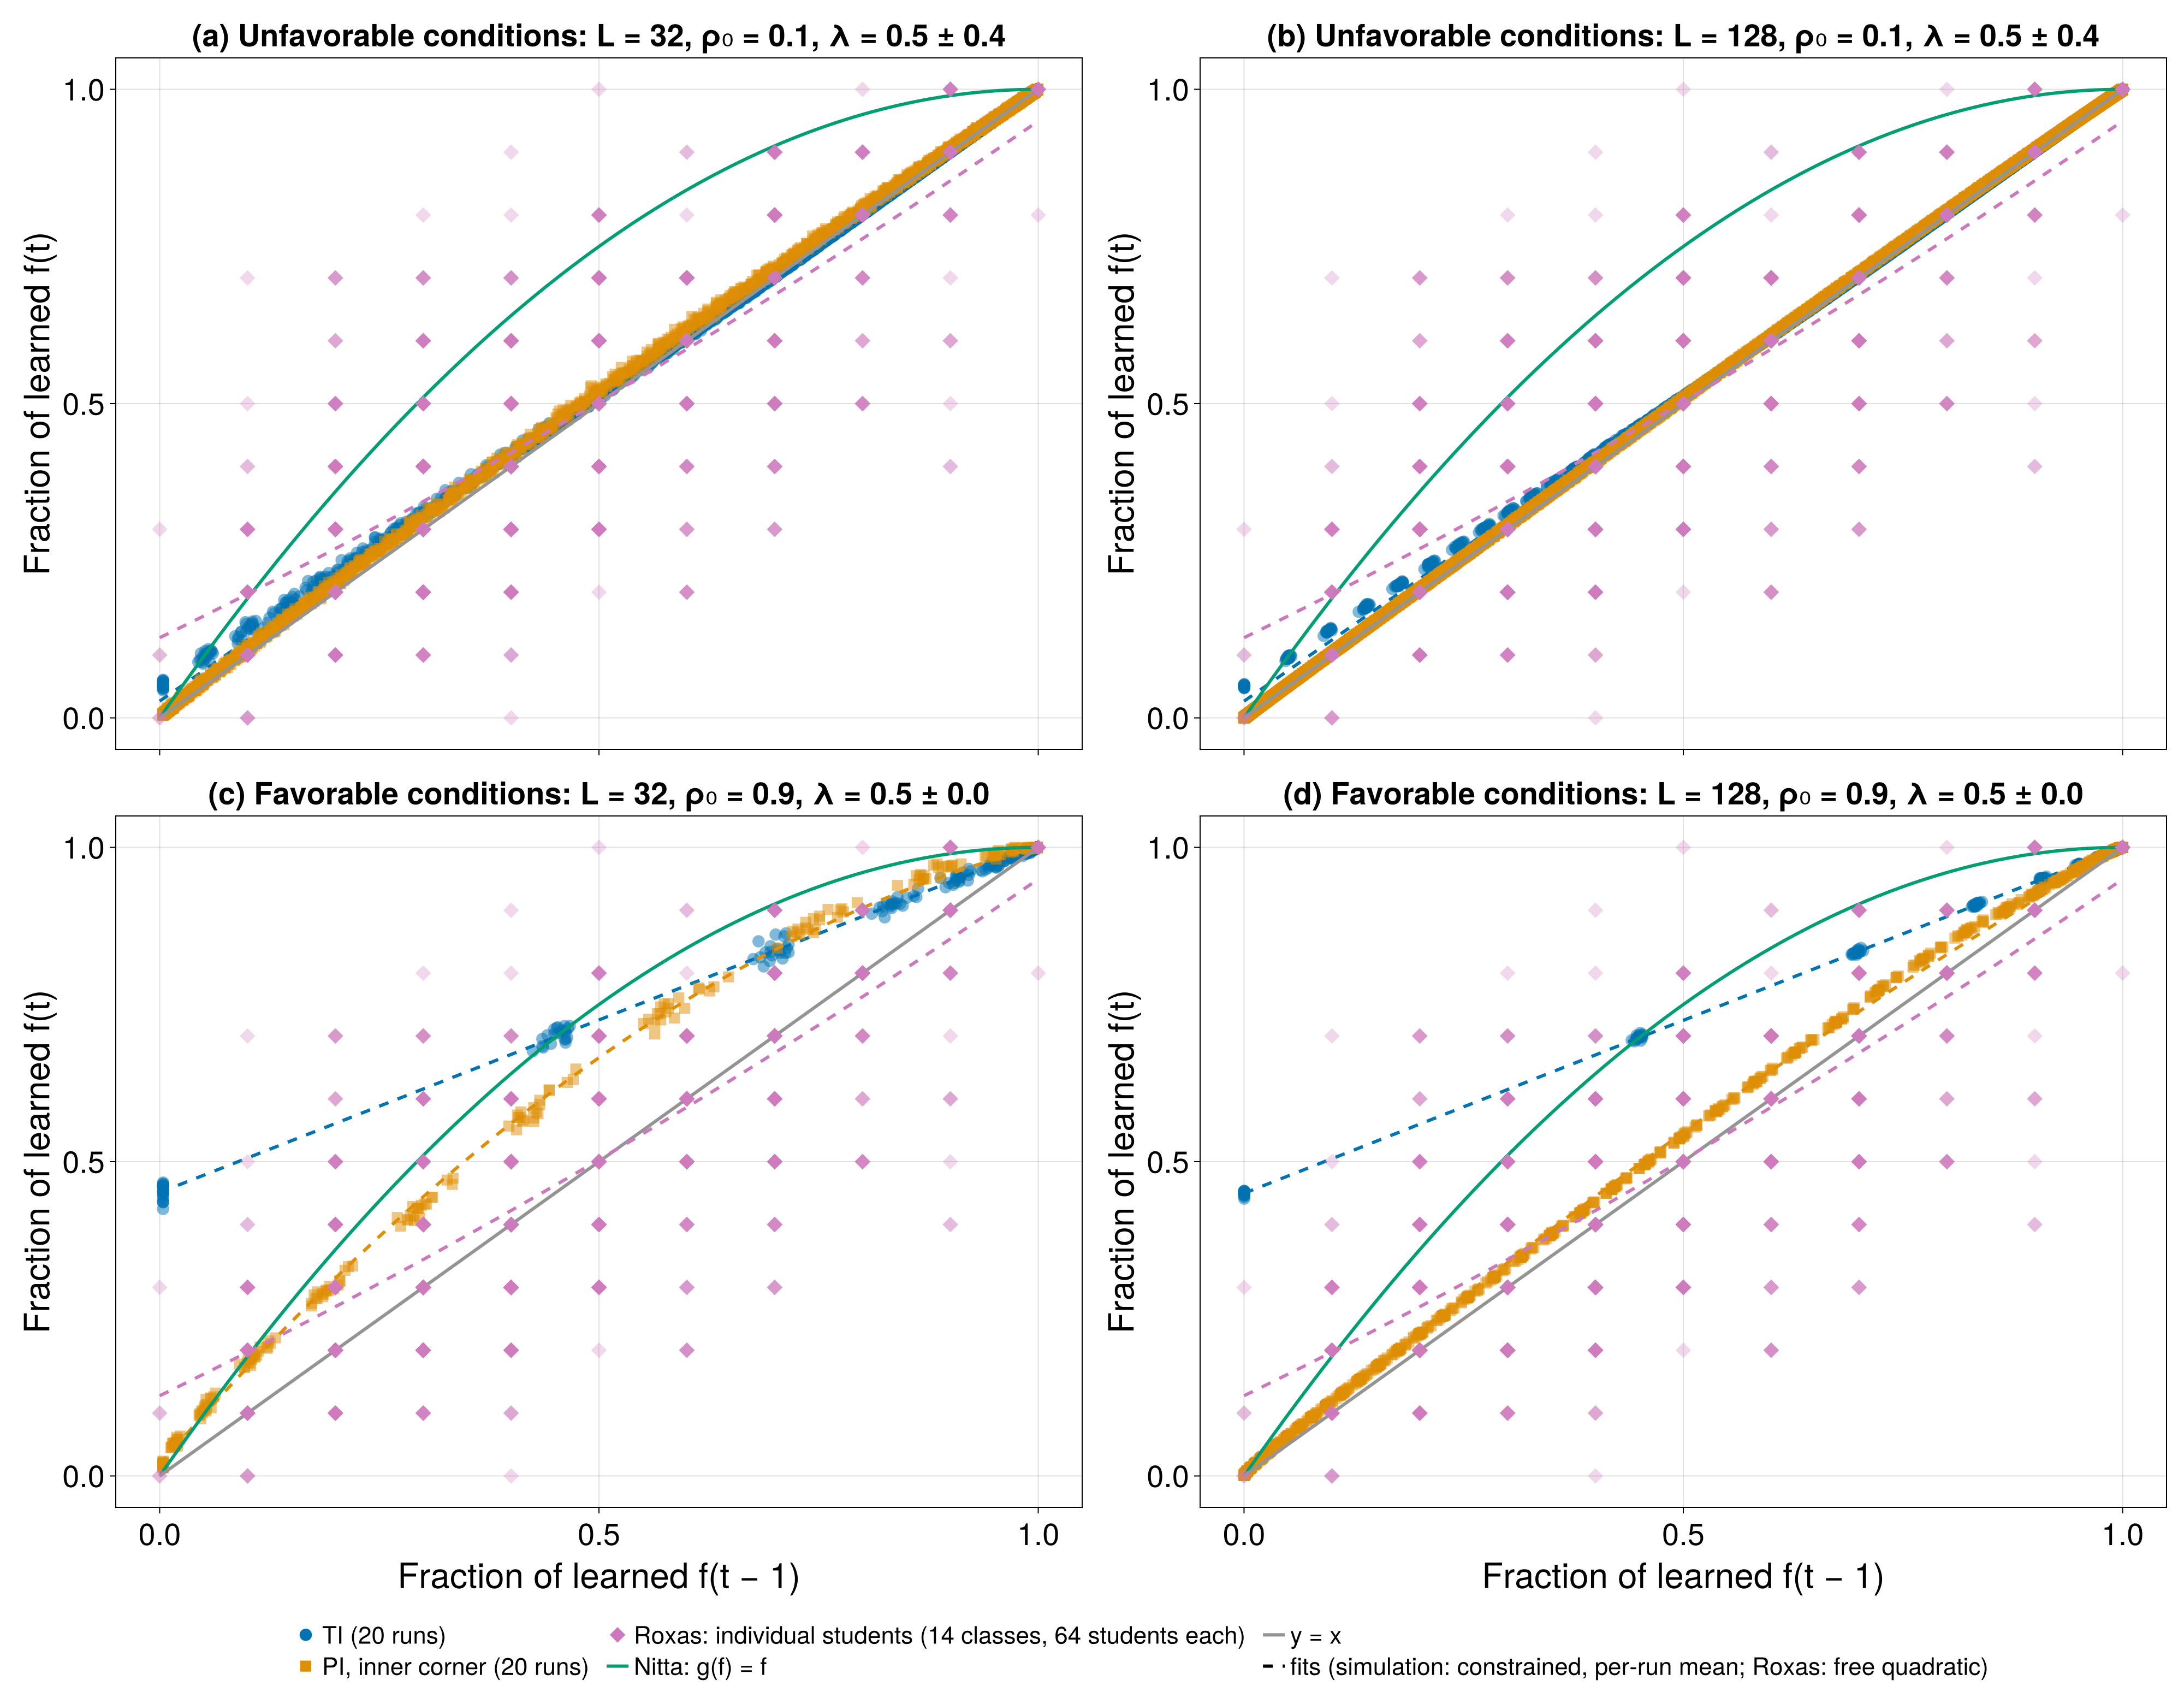
\includegraphics[width=0.95\textwidth]{figs/figure6-v2.png}
        \caption{
        Return map of the learned agent fraction, $f(t)$ against $f(t-1)$, in unfavorable conditions ($\rho_0=0.1$, $\delta\lambda=0.4$; top row) and favorable conditions ($\rho_0=0.9$, $\delta\lambda=0$; bottom row), for $L=32$ (left) and $L=128$ (right), so that panels in the same row differ only in system size.
        Blue circles represent the broadcast (TI) regime and orange squares the nearest-neighbor (PI) regime with the inner corner arrangement, 20 runs each.
        Pink diamonds represent individual students in the empirical data of Roxas (fourteen classes of 64 students); darker diamonds indicate overlapping points.
        Dashed lines show the fitted return maps: for the simulations, the constrained broadcast and nearest-neighbor forms with coefficients averaged over separate fits to each run (Table~\ref{tbl:returnmapfits}); for the empirical data, a free quadratic.
        The green line represents the prediction of~\citet{nitta2019mathematical} and the gray line represents $y=x$.
        }
        \label{fig:Return map}
    \end{figure}

    \begin{figure}[htbp]
        \centering
        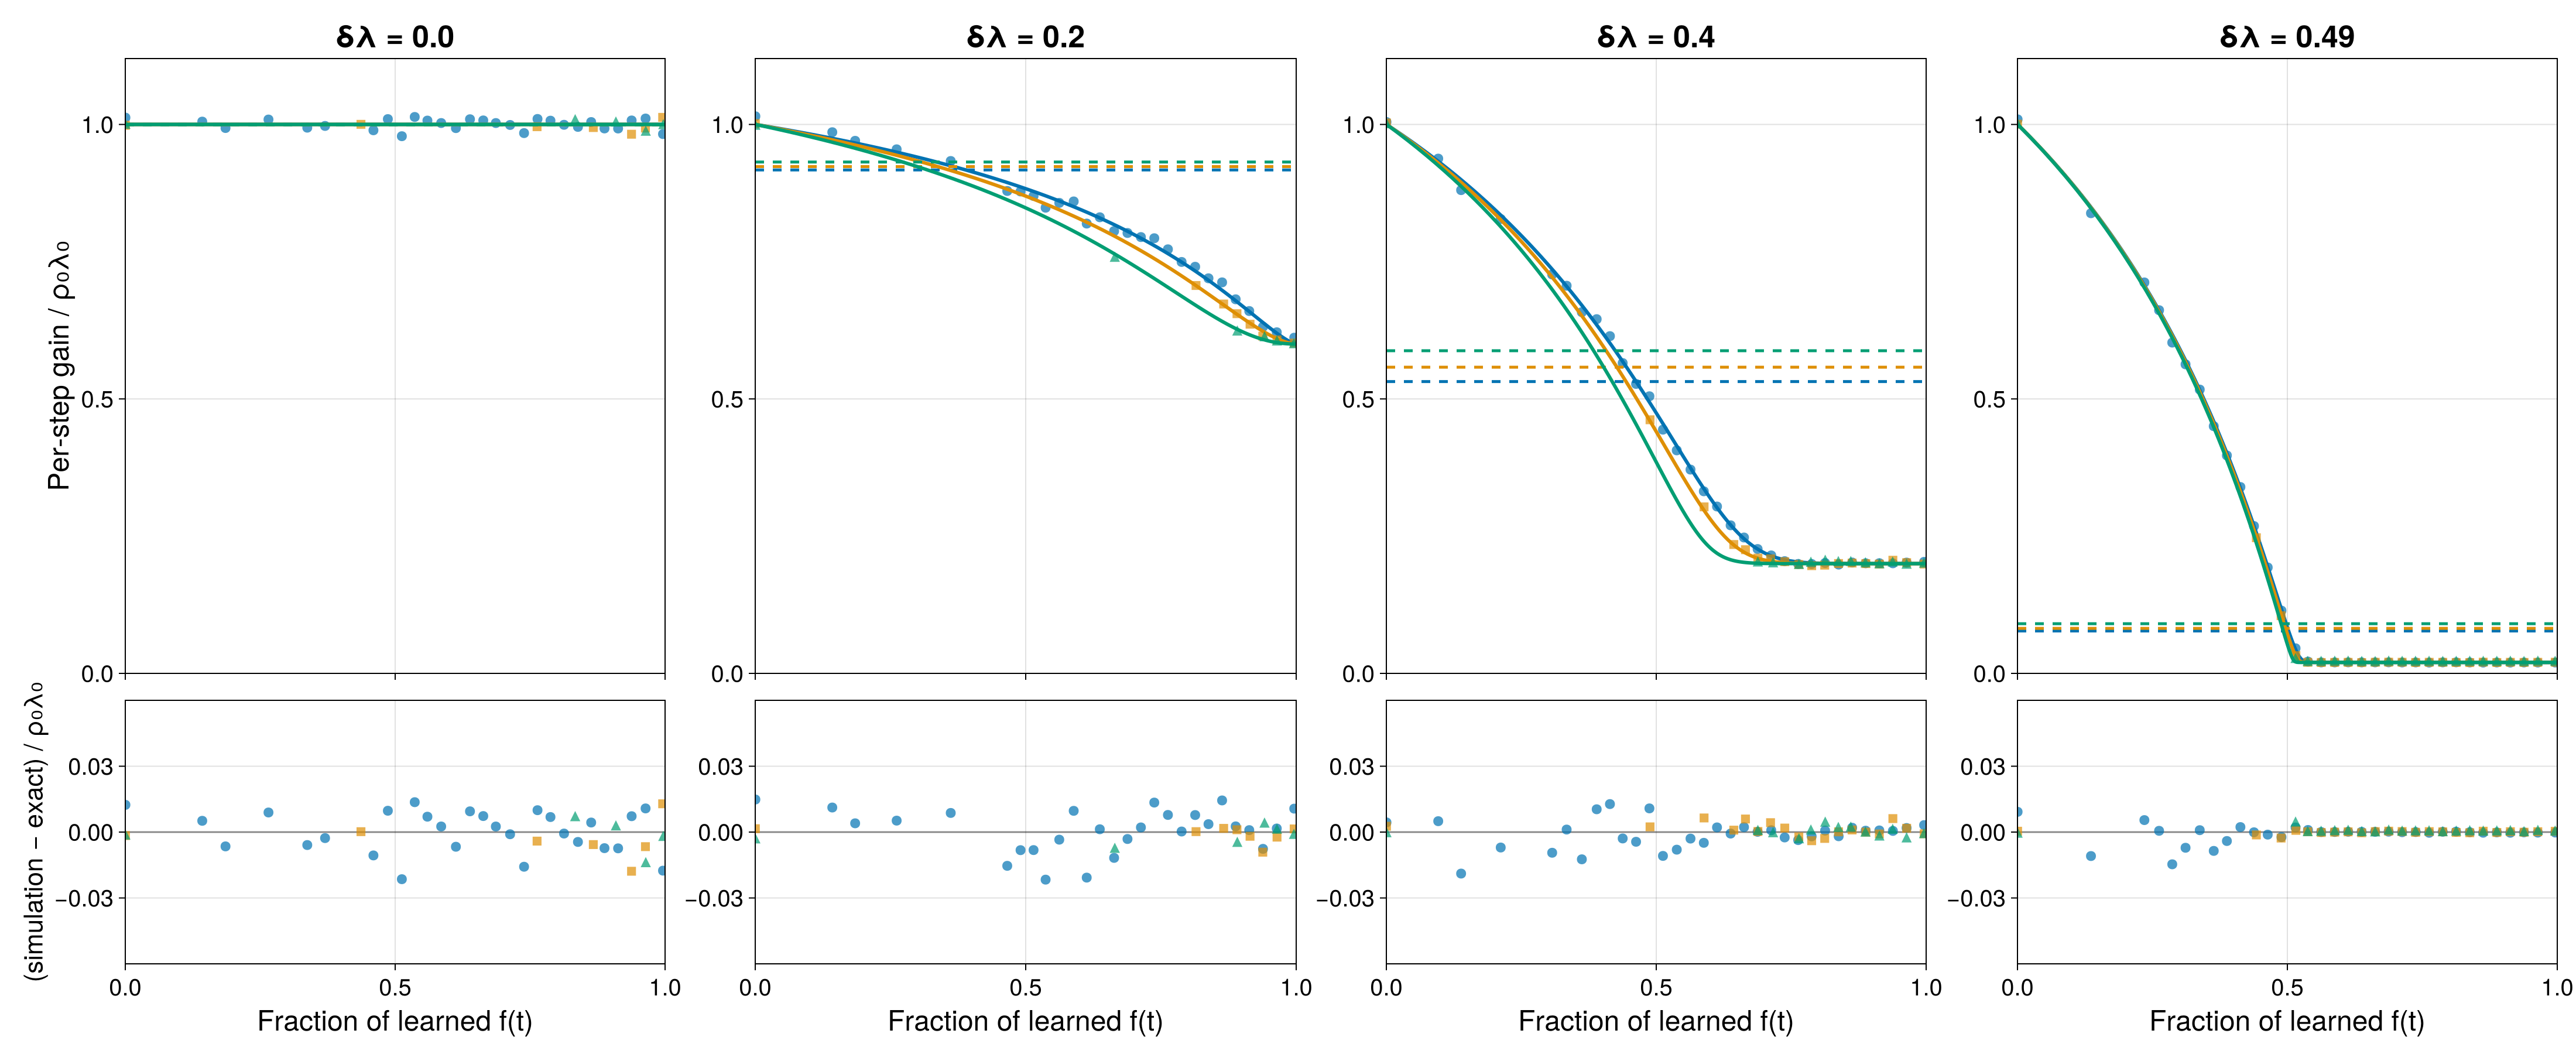
\includegraphics[width=\textwidth]{figs/figure-ti-gain.png}
        \caption{Per-step gain of the broadcast regime, normalized by $\rho_0\lambda_0$, against the fraction of learned agents, for $L=128$, $\delta\lambda=0$, $0.2$, $0.4$, and $0.49$ (left to right), and $\rho_0=0.1$ (blue circles), $0.5$ (orange squares), and $0.9$ (green triangles). Symbols: simulation (agents newly learned divided by agents unlearned, summed over 20 runs within bins of $f$); solid lines: exact gain, Eq.~\eqref{eq:ti-exact-gain}; dashed lines: fitted constant $a_0$. Bottom row: simulation minus exact gain.}
        \label{fig:ti gain}
    \end{figure}

    \begin{figure}[htbp]
        \centering
        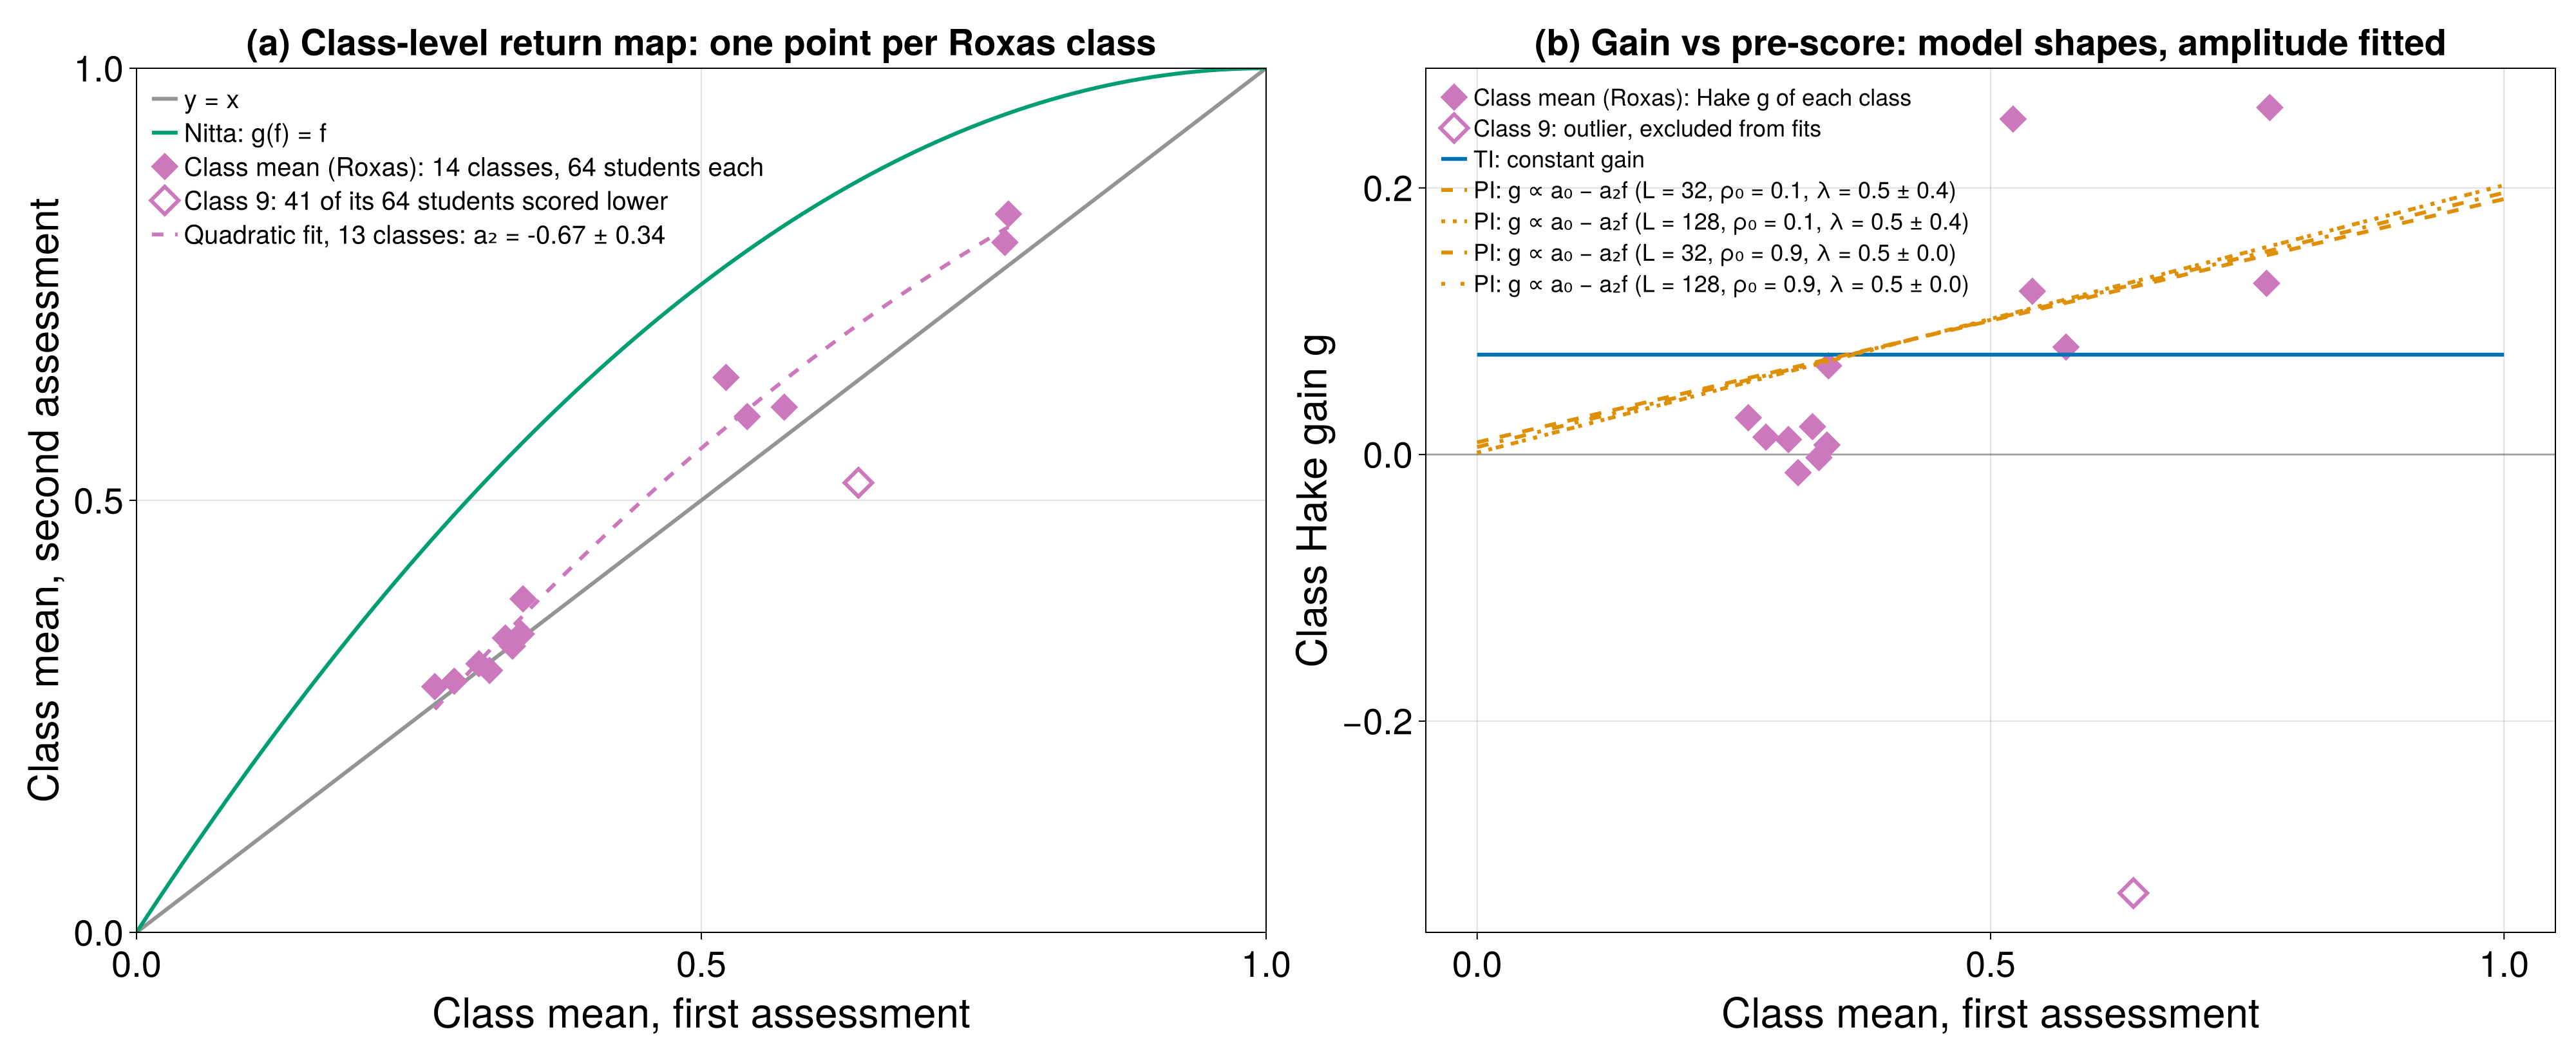
\includegraphics[width=0.95\textwidth]{figs/figure6b.png}
        \caption{
        Class-level comparison with the empirical data of Roxas (fourteen classes of 64 students; one point per class, using the class mean scores).
        (a)~Class mean post-test score against class mean pre-test score. The gray line represents $y=x$, the green line the prediction of~\citet{nitta2019mathematical}, and the dashed line a free quadratic fitted to the class means (class 9 excluded), with $a_2=-0.67\pm0.34$.
        (b)~Class Hake gain against class mean pre-test score, with the gain shapes of the two regimes, each with one fitted amplitude: constant gain (broadcast, solid blue) and $g\propto a_0-a_2f$ (nearest-neighbor, orange) with the coefficients of each of the four cases in Fig.~\ref{fig:Return map}; the four curves nearly coincide because $a_0\ll|a_2|$ in every case.
        The open marker is class 9, excluded from the fits as an outlier.
        }
        \label{fig:Return map class}
    \end{figure}

    % \begin{table*}[htbp]
    % \caption{Return-map fit statistics for the broadcast (TI) and nearest-neighbor (PI) regimes and the empirical data. Simulation fits impose $h(1)=1$; the broadcast form $h(f)=f+a_0(1-f)$ has the single free parameter $a_0$, and the nearest-neighbor form $h(f)=f+(1-f)(a_0-a_2 f)$ has free parameters $a_0$ and $a_2$. The empirical fit is a free quadratic $h(f)=a_0+a_1 f+a_2 f^2$. Uncertainties are one standard error from the Levenberg--Marquardt fit; $N_{\rm pts}$ is the number of $(f_{t-1},f_t)$ pairs.}
    % \label{tbl:returnmapfits}
    % \begin{tabular*}{\tblwidth}{@{}LLLLLL@{}}
    % \toprule
    % Dataset & $a_0$ & $a_1$ & $a_2$ & $R^2$ & $N_{\rm pts}$ \\
    % \midrule
    % TI, large ($L=128$) & $0.0267\pm0.0001$ & N/A & N/A & $0.9997$ & $19054$ \\
    % PI, large ($L=128$) & $(1.6\pm0.2)\times10^{-4}$ & N/A & $-0.0358\pm0.0001$ & $1.0000$ & $6011$ \\
    % TI, small ($L=32$) & $0.4454\pm0.0013$ & N/A & N/A & $0.9979$ & $257$ \\
    % PI, small ($L=32$) & $0.0189\pm0.0012$ & N/A & $-0.6247\pm0.0058$ & $0.9993$ & $252$ \\
    % Empirical (Roxas) & $0.128\pm0.020$ & $0.680\pm0.088$ & $0.142\pm0.086$ & $0.633$ & $896$ \\
    % \bottomrule
    % \end{tabular*}
    % \end{table*}

    \begin{table*}[htbp]
    \caption{Return-map fit statistics for the broadcast (TI) and nearest-neighbor (PI, inner corner) regimes in the four cases of Fig.~\ref{fig:Return map}, and for the empirical data.
    Simulation fits impose $h(1)=1$; the broadcast form $h(f)=f+a_0(1-f)$ has the single free parameter $a_0$, and the nearest-neighbor form $h(f)=f+(1-f)(a_0-a_2 f)$ has free parameters $a_0$ and $a_2$.
    Each of the 20 runs is fitted separately, since consecutive points of one run are correlated; simulation coefficients are the mean over runs $\pm$ the standard error of the mean, and $R^2$ is the mean over runs.
    The empirical fits are free quadratics $h(f)=a_0+a_1 f+a_2 f^2$ to the individual students (896 pre/post pairs) and to the class means (thirteen classes, class 9 excluded), with one standard error from the fit. For $\delta\lambda>0$ the broadcast $a_0$ is an effective constant (Table~\ref{tbl:ti gain}).}
    \label{tbl:returnmapfits}
    \begin{tabular*}{\tblwidth}{@{}LLLLLLLL@{}}
    \toprule
    Dataset & $L$ & $\rho_0$ & $\delta\lambda$ & $a_0$ & $a_1$ & $a_2$ & $R^2$ \\
    \midrule
    TI & $32$ & $0.1$ & $0.4$ & $0.0266\pm0.0004$ & -- & -- & $0.9997$ \\
    TI & $128$ & $0.1$ & $0.4$ & $0.02658\pm0.00008$ & -- & -- & $0.9997$ \\
    TI & $32$ & $0.9$ & $0$ & $0.451\pm0.002$ & -- & -- & $0.9989$ \\
    TI & $128$ & $0.9$ & $0$ & $0.4497\pm0.0006$ & -- & -- & $0.9999$ \\
    PI & $32$ & $0.1$ & $0.4$ & $(3.6\pm0.2)\times10^{-3}$ & -- & $-0.0716\pm0.0013$ & $1.0000$ \\
    PI & $128$ & $0.1$ & $0.4$ & $(2.3\pm0.2)\times10^{-4}$ & -- & $-0.0343\pm0.0002$ & $1.0000$ \\
    PI & $32$ & $0.9$ & $0$ & $0.0184\pm0.0006$ & -- & $-0.625\pm0.005$ & $0.9994$ \\
    PI & $128$ & $0.9$ & $0$ & $(1.24\pm0.02)\times10^{-3}$ & -- & $-0.1836\pm0.0003$ & $0.9997$ \\
    \midrule
    Empirical, students & -- & -- & -- & $0.128\pm0.020$ & $0.680\pm0.088$ & $0.142\pm0.086$ & $0.633$ \\
    Empirical, class means & -- & -- & -- & $-0.17\pm0.08$ & $1.79\pm0.35$ & $-0.67\pm0.34$ & $0.985$ \\
    \bottomrule
    \end{tabular*}
    \end{table*}

    \begin{table}[htbp]
    \caption{Constant broadcast gain $a_0$ of Eq.~\eqref{eq:ti-return-map} compared with the exact gain $g$ of Eq.~\eqref{eq:ti-exact-gain}, for $L=128$: the fitted $a_0$ (mean over 20 runs) relative to $\rho_0\lambda_0$; the ratio $g_{\rm start}/g_{\rm end}$ of the exact gain at the start of the relaxation, $g(0)=\rho_0\lambda_0$, to its final value, $\lim_{t\to\infty}g(t)=\rho_0(\lambda_0-\delta\lambda)$; and the largest relative difference between the exact and the constant gain over the relaxation, $\max_t|g(t)-a_0|/a_0$. Ranges are over $\rho_0=0.1$, $0.5$, and $0.9$.}
    \label{tbl:ti gain}
    \begin{tabular*}{\tblwidth}{@{}l@{\extracolsep{\fill}}ccc@{}}
    \toprule
    $\delta\lambda$ & $a_0/\rho_0\lambda_0$ & $g_{\rm start}/g_{\rm end}$ & $\max_t|g(t)-a_0|/a_0$ \\
    \midrule
    $0$ & $1.00$ & $1$ & $\leq0.001$ \\
    $0.2$ & $0.92$--$0.93$ & $1.67$ & $0.35$--$0.36$ \\
    $0.4$ & $0.53$--$0.59$ & $5$ & $0.70$--$0.88$ \\
    $0.45$ & $0.32$--$0.37$ & $10$ & $1.7$--$2.1$ \\
    $0.49$ & $0.08$--$0.09$ & $50$ & $10$--$12$ \\
    \bottomrule
    \end{tabular*}
    \end{table}

% Forces the last two figures (which otherwise drift past the bibliography
% to the very last page -- see preamble note) to resolve here instead.
\clearpage
\section{Summary and Conclusion}

We have presented a probabilistic cellular automata (pCA) model for investigating the collective relaxation dynamics of a heterogeneous agent population under two distinct interaction topologies: a broadcast regime, analogous to traditional instruction, and a nearest-neighbor regime, analogous to peer instruction.
The model is defined on a two-dimensional rectangular lattice, with each agent assigned a binary state and an individual learning rate $\lambda$ drawn from a two-level heterogeneous distribution parameterized by $\delta\lambda$.

The two regimes exhibit qualitatively distinct relaxation dynamics.
The broadcast regime drives a rapid early onset of transitions across the agent population, but is sensitive to agent heterogeneity: high $\delta\lambda$ produces a pronounced two-stage relaxation, with the fast initial stage driven by the high-$\lambda$ subpopulation and the slow residual stage governed by the low-$\lambda$ subpopulation.
The nearest-neighbor regime exhibits local propagation dynamics, producing a gradual initial increase in the learned fraction followed by a sharp rise as the number of active interfaces grows.
This regime is more robust to agent heterogeneity, exhibiting only a gradual delay in the relaxation curve across all $\delta\lambda$ values considered, with no qualitative change in curve shape apart from a slower final approach to the fully learned state at the strongest heterogeneity.

In terms of the total relaxation time $t_{\rm max}$, the broadcast regime relaxes faster for larger lattice side lengths at low heterogeneity, and the nearest-neighbor regime for smaller lattice side lengths and at high heterogeneity, where its lead in absolute time is much larger; as ratios, the differences in either direction are comparable.
The time $t_{95}$ for $95\%$ of agents to learn gives a different picture: for the larger lattice side length it is shorter in the broadcast regime up to moderate heterogeneity, because the broadcast $t_{\rm max}$ is set by the slowest of $N$ independently transitioning agents, whereas the nearest-neighbor front leaves few agents behind.
These complementary strengths, the broadcast regime bringing most agents to the learned state quickly and the nearest-neighbor regime leaving few behind and remaining robust under heterogeneity, suggest that a combination of both regimes may outperform either one alone; this remains a hypothesis to be tested with a model that combines the two.

The fixed-point structure of the relaxation dynamics was further characterized through a return map analysis, from which class-level Hake gains were obtained by fitting the simulated return maps.
The broadcast regime yields a constant gain $g(f)=a_0$, exact for a homogeneous population and an effective average under heterogeneity, while the nearest-neighbor regime gives a quadratic return map and hence a linear gain $g(f)=a_0-a_2f$, consistent with existing theoretical predictions~\citep{nitta2019mathematical}.
The return map approach was also applied to empirical classroom data, where, once within-class differences are averaged out, the class-level gain increases with the pre-test score, consistent with the nearest-neighbor regime, and we propose it as a practical method for empirically estimating class-level Hake gains from pre- and post-test results.

While the present model is necessarily simplified, it captures the essential dynamical features of both interaction regimes and provides a tractable framework for investigating the effects of system size, coupling strength, and agent heterogeneity on collective relaxation dynamics.
A central simplifying assumption warrants emphasis as a limitation: each agent has a single monotonic absorbing state, so once an agent learns it can never revert. The model therefore admits no forgetting, regression, or erroneous learning, and cannot reproduce the score decreases from pre- to post-test that are present in real classroom data (and, indeed, in the empirical dataset compared against in Section~\ref{sec:rnd}). This monotonic absorbing-state assumption is a major constraint on the realism of the model and, together with the binary-state and isotropic-coupling simplifications, bounds the extent to which the model can be expected to match empirical classroom dynamics.
Future extensions of the model could incorporate continuous-valued agent states to capture aptitude similarity effects and to admit non-monotonic dynamics such as forgetting and regression, anisotropic coupling to account for spatial orientation in the classroom, a varied mean learning rate $\lambda_0$, and a mixed-regime model that explicitly combines broadcast and nearest-neighbor phases within a single simulation, which would directly test the combined strategy hypothesized above.

\section*{Code availability}
The cellular automata simulation and analysis code used to generate and process the data in this study is available at [repository URL and Zenodo DOI to be added].

\section*{Data availability}
The simulation output supporting the findings of this study, including the random seed of every run, is available at [Zenodo DOI to be added]. The empirical classroom data are available from the corresponding author upon reasonable request.

% Numbered list
% Use the style of numbering in square brackets.
% If nothing is used, default style will be taken.
%\begin{enumerate}[a)]
%\item 
%\item 
%\item 
%\end{enumerate}  

% Unnumbered list
%\begin{itemize}
%\item 
%\item 
%\item 
%\end{itemize}  

% Description list
%\begin{description}
%\item[]
%\item[] 
%\item[] 
%\end{description}  

% \clearpage %%Remove this from your manuscript

% % Figure
% \begin{figure}%[]
%   \centering
% %    \includegraphics{}
%     \caption{}\label{fig1}
% \end{figure}

% Uncomment and use as the case may be
%\begin{theorem} 
%\end{theorem}

% Uncomment and use as the case may be
%\begin{lemma} 
%\end{lemma}

%% The Appendices part is started with the command \appendix;
%% appendix sections are then done as normal sections
%% \appendix

% \section{}\label{}

\appendix
\section{Total relaxation time and time to 95\% learned}\label{app:t95}

Fig.~\ref{fig:t95 vs tmax} shows $t_{\rm max}$ and $t_{95}$ as functions of heterogeneity, including $\delta\lambda=0.45$ and $0.49$, which Fig.~\ref{fig:Params effect summary t} omits, together with their run-to-run spread.

    \begin{figure}[htbp]
        \centering
        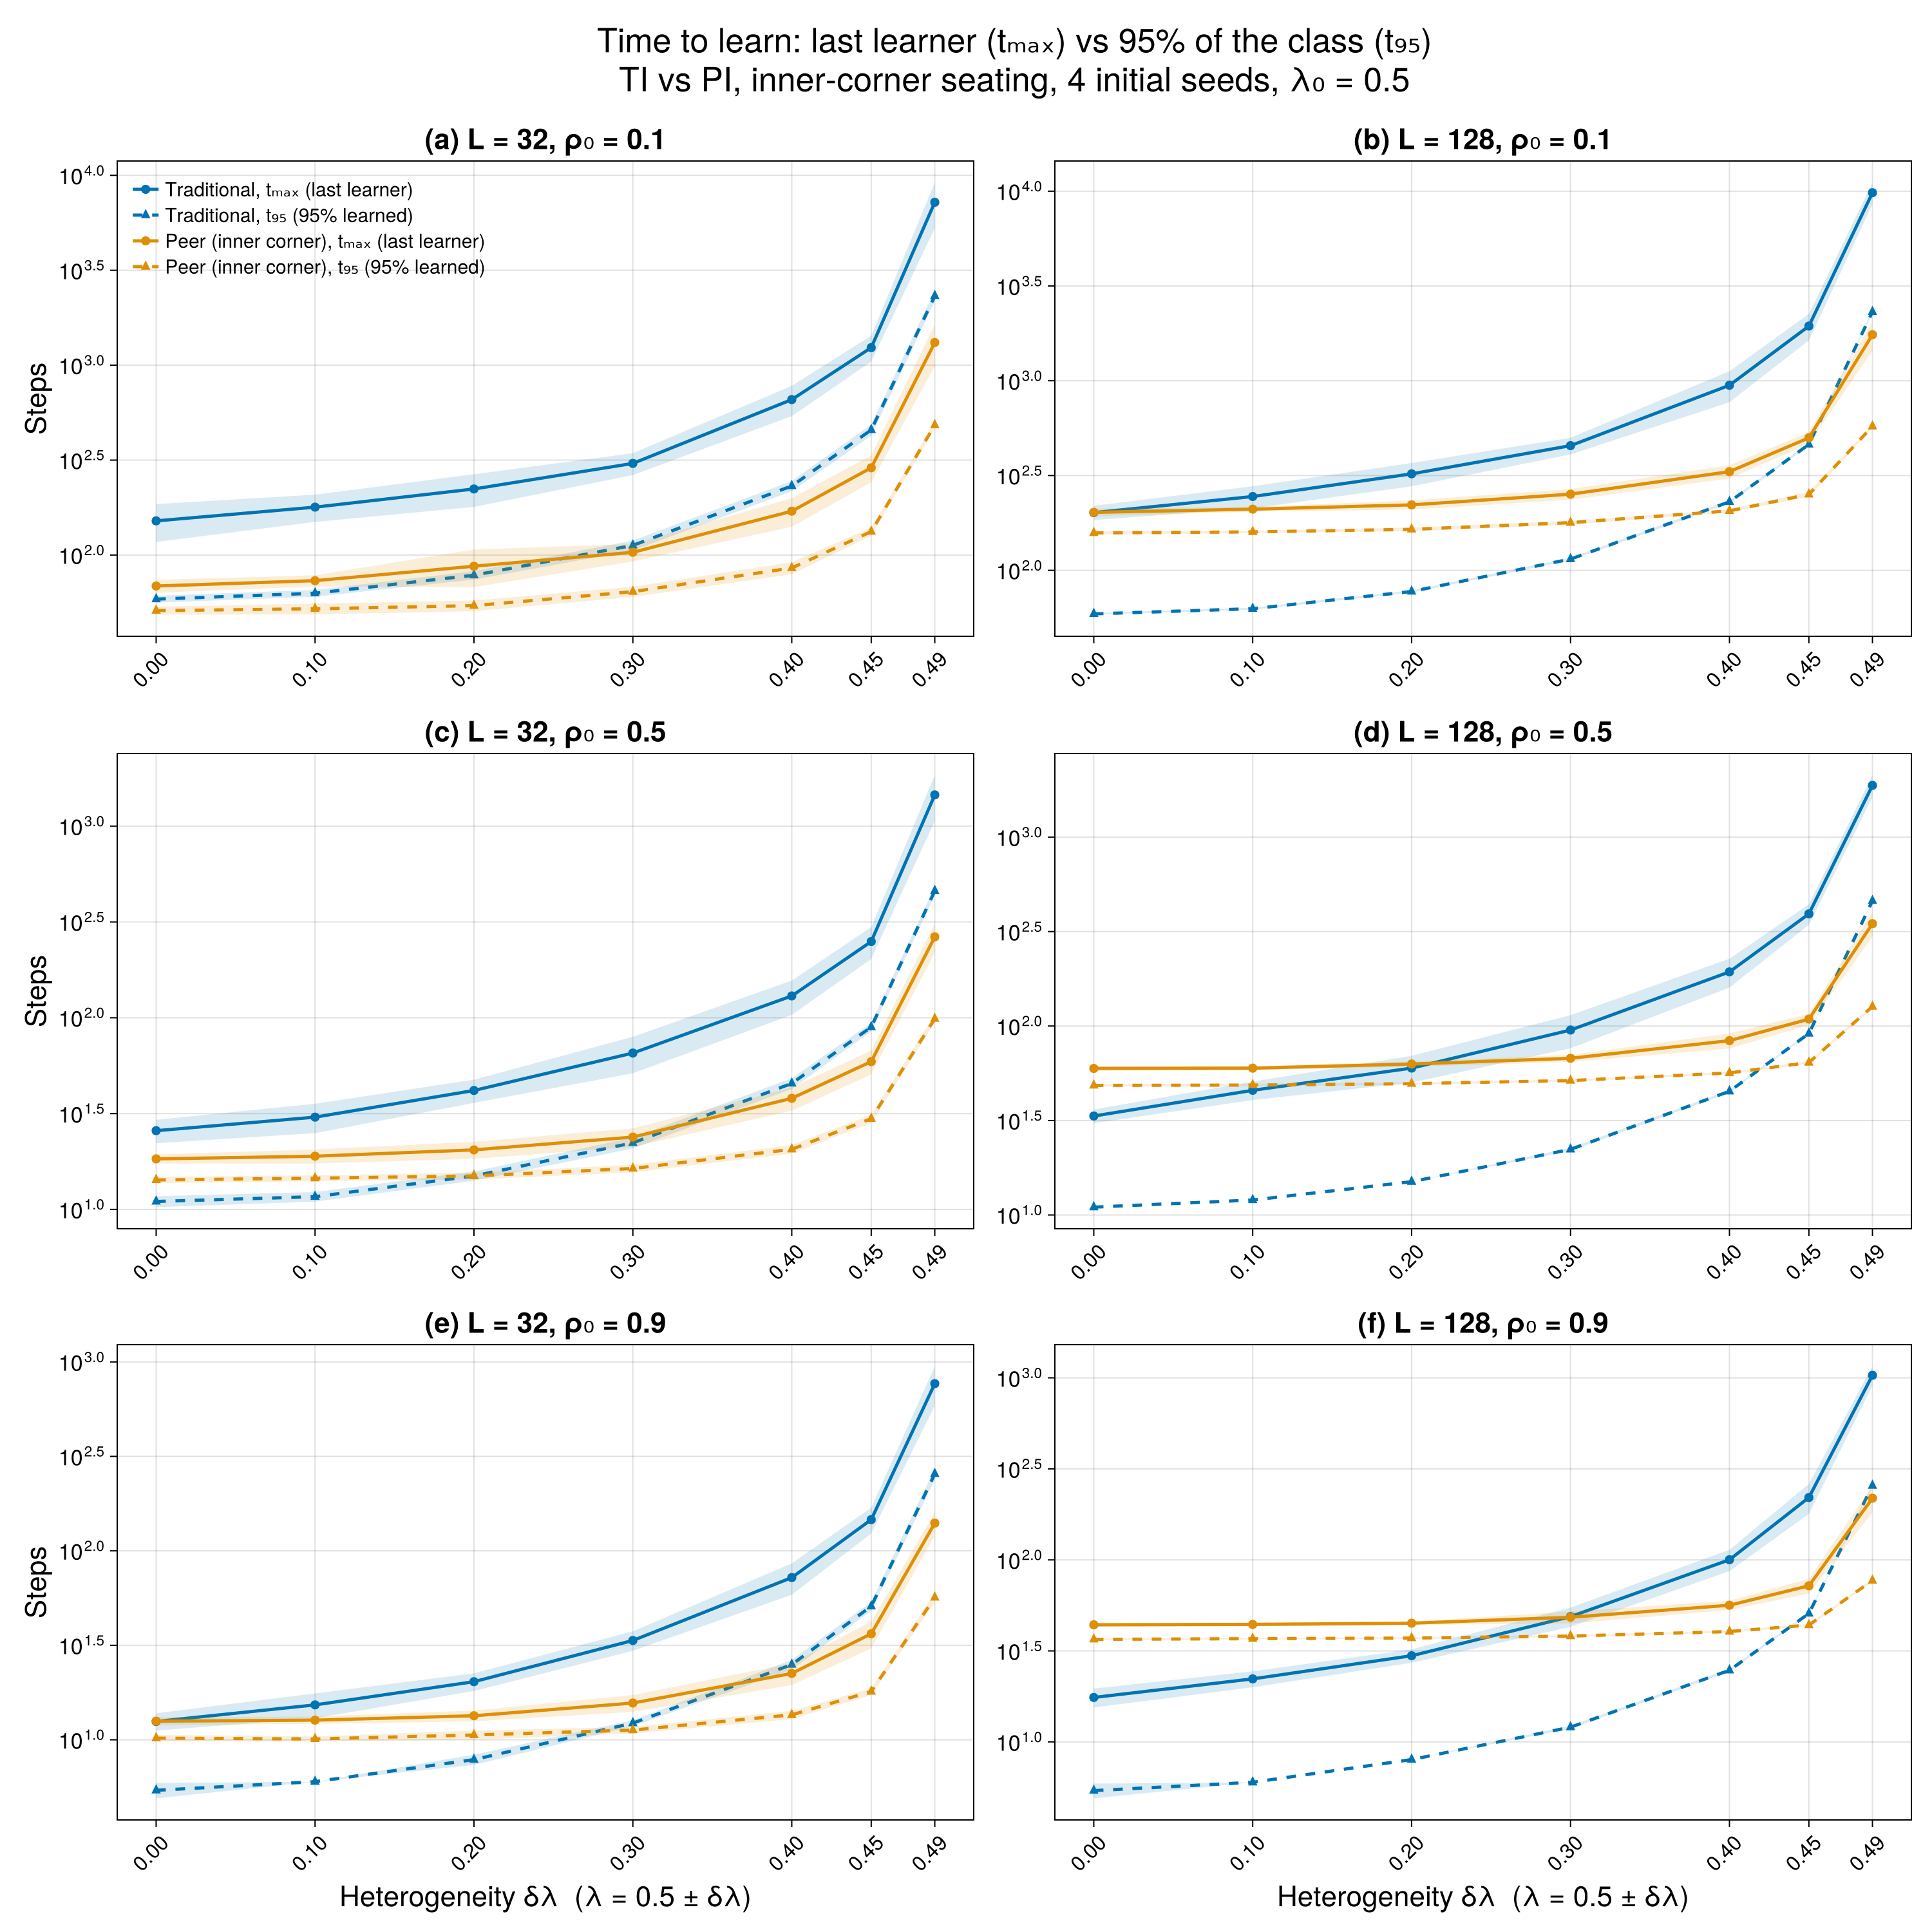
\includegraphics[width=0.9\textwidth]{figs/figure5b-t95.png}
        \caption{
        Total relaxation time $t_{\rm max}$ (solid lines, last agent learned) and $t_{95}$ (dashed lines, $95\%$ of agents learned) as functions of heterogeneity $\delta\lambda$, for the broadcast (blue) and nearest-neighbor (orange, inner corner seating) regimes, at $L=32$ (left column) and $L=128$ (right column) and $\rho_0=0.1$, $0.5$, and $0.9$ (rows), with $\lambda_0=0.5$ and four initially learned agents. Lines show the mean and bands one standard deviation over 20 runs; the vertical axis is logarithmic.
        }
        \label{fig:t95 vs tmax}
    \end{figure}

\section{Return-map coefficients versus lattice size}\label{app:coefs vs L}

Fig.~\ref{fig:coefs vs L} shows the return-map coefficients as functions of the lattice side $L$ at fixed coupling strength and heterogeneity, for the inner corner arrangement.
Heterogeneity values $\delta\lambda\geq0.45$ are omitted because the quadratic nearest-neighbor form no longer describes the two-stage relaxation there.
Solid lines use four initially learned agents, as in the rest of this work; dashed lines hold the initial learned fraction fixed at that of the $L=32$ lattice ($4L^2/32^2$ initially learned agents).
The nearest-neighbor $a_0$ is the intercept of the return map at $f=0$, which few points constrain, so $|a_2|$ is the more reliable measure of the size dependence.

\begin{figure}[htbp]
    \centering
    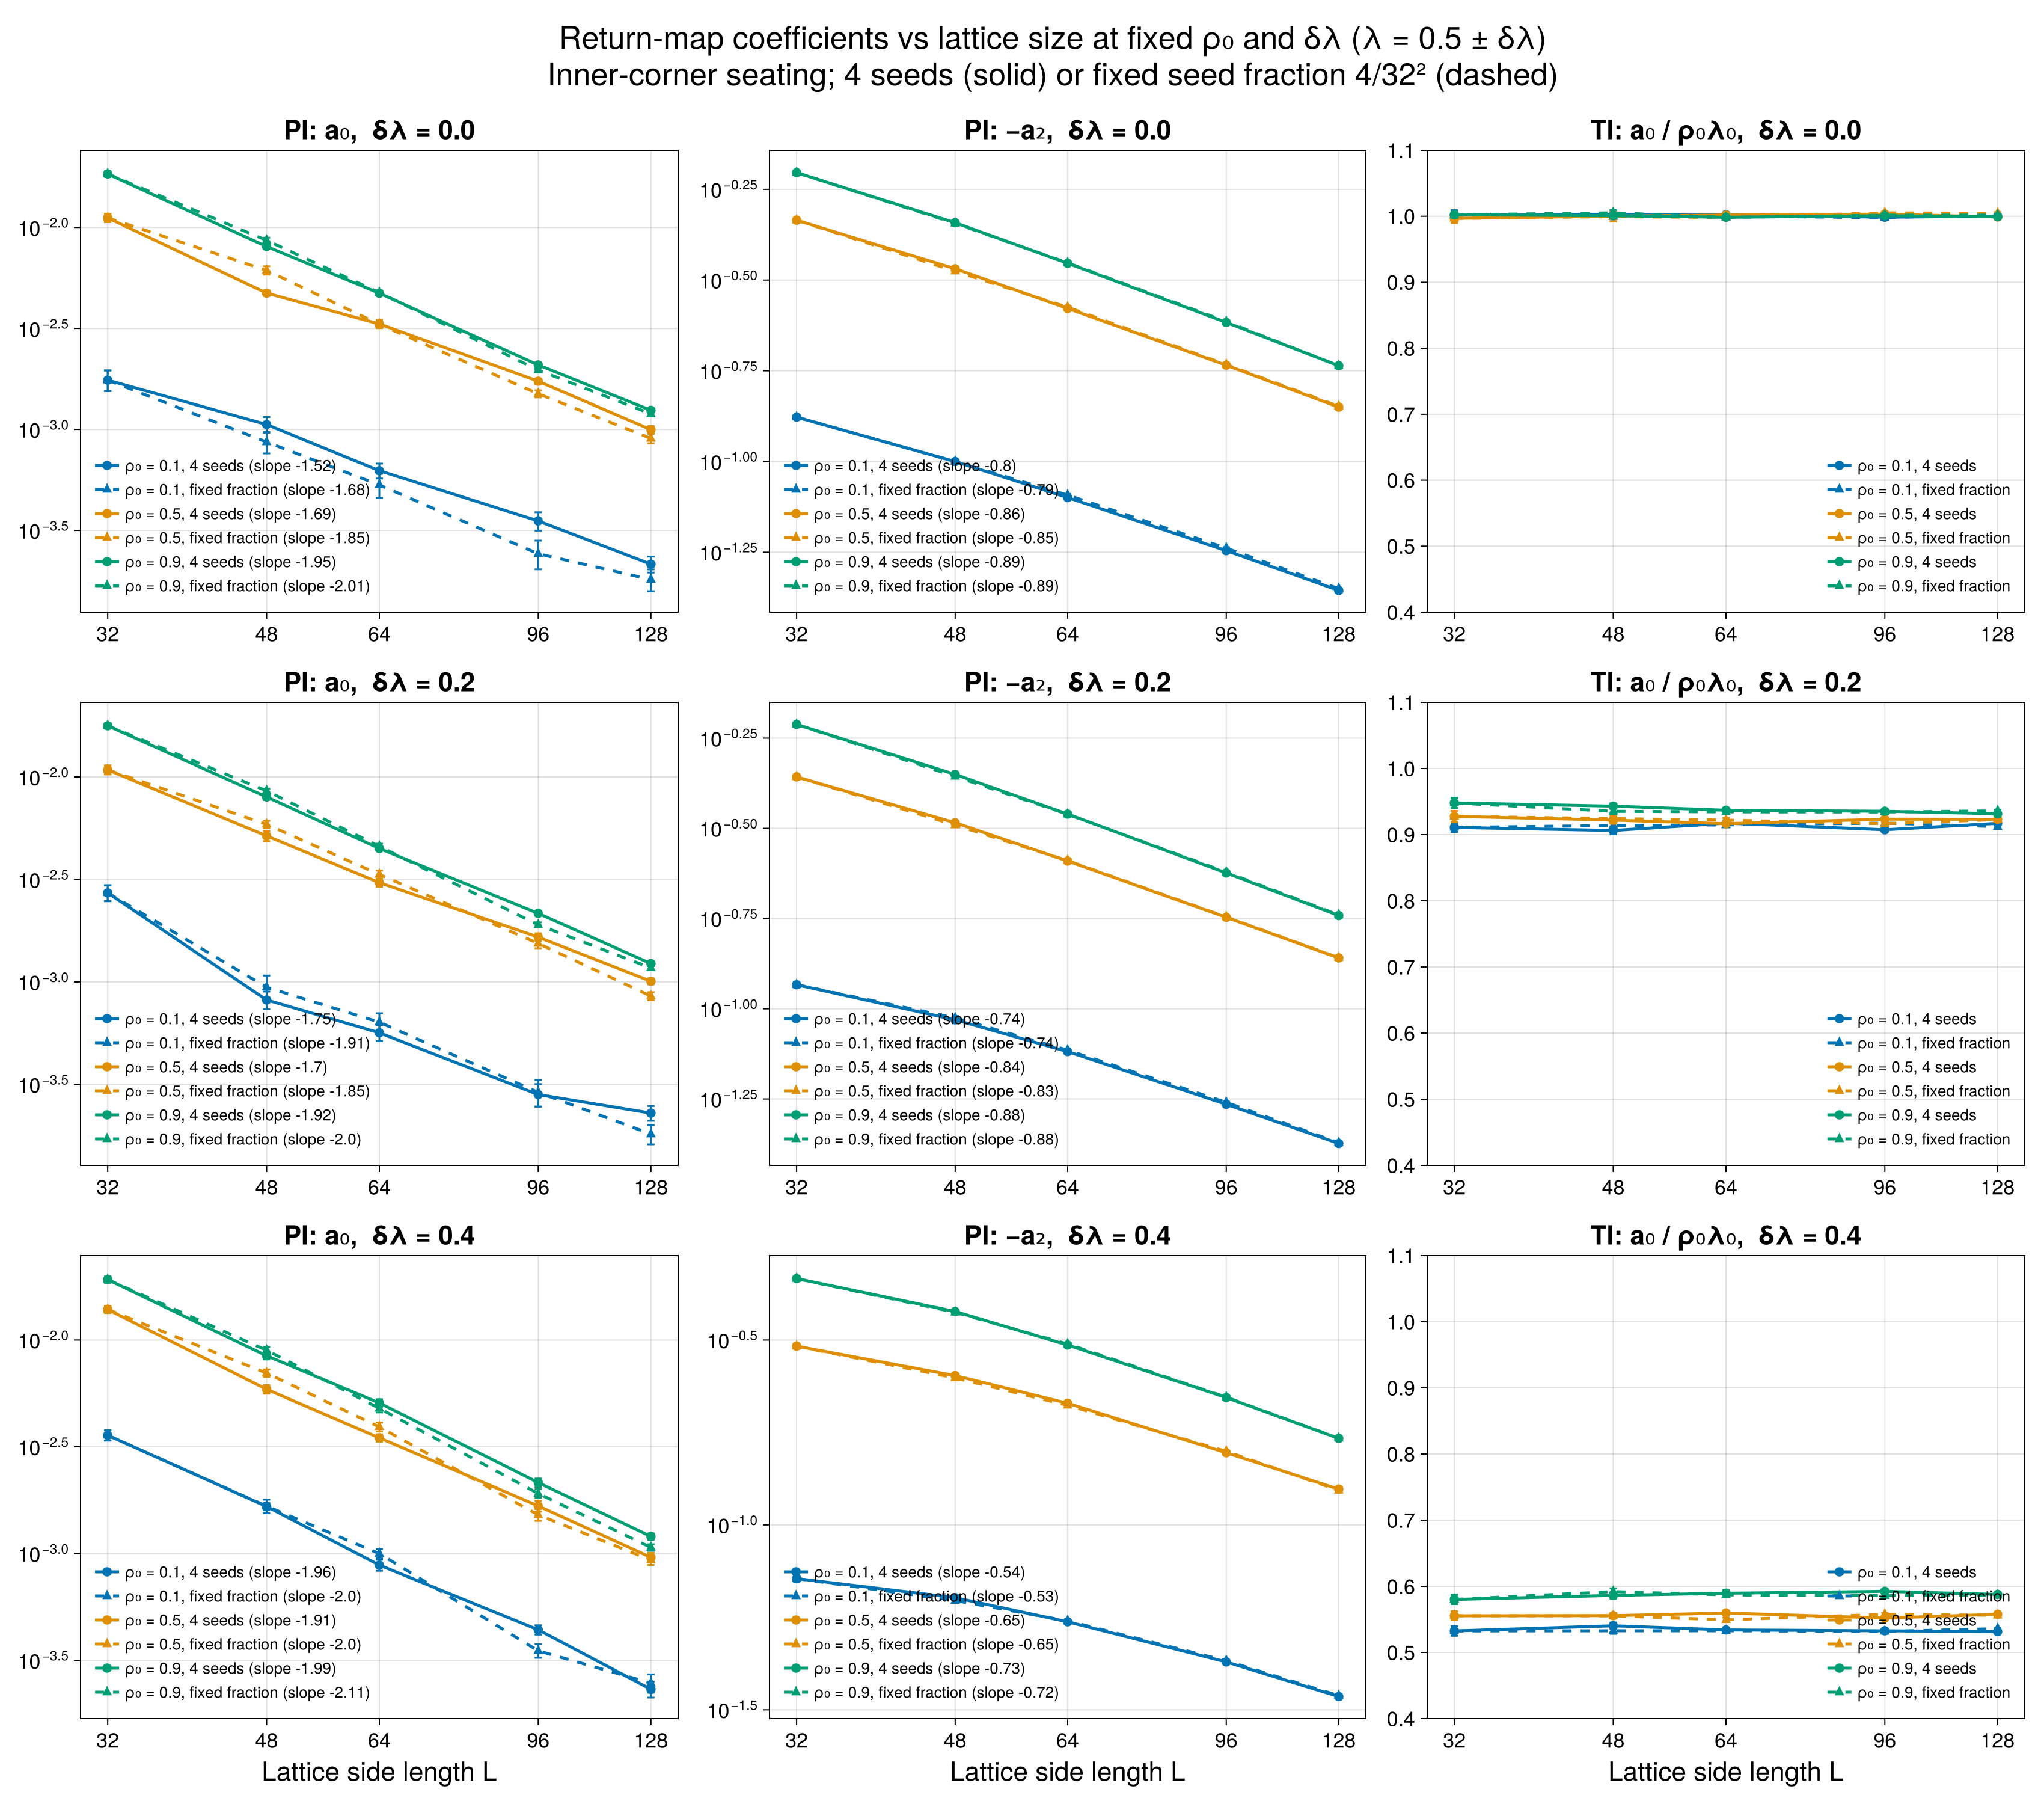
\includegraphics[width=\textwidth]{figs/figureA1.png}
    \caption{Return-map coefficients against lattice side $L$ (logarithmic axes for the nearest-neighbor coefficients) for $\rho_0\in\{0.1,0.5,0.9\}$ (colors) and $\delta\lambda\in\{0,0.2,0.4\}$ (rows); mean over 20 runs, each fitted separately, $\pm$ the standard error of the mean.
    Left: nearest-neighbor $a_0$. Center: nearest-neighbor $-a_2$. Right: broadcast $a_0$, normalized by $\rho_0\lambda_0$.
    Solid lines: four initially learned agents; dashed lines: fixed initial learned fraction. The legends give the log--log slopes.}
    \label{fig:coefs vs L}
\end{figure}

\section{Size scaling at a fixed initial learned fraction}\label{app:seed density}

Fig.~\ref{fig:seed density} compares the nearest-neighbor $t_{\rm max}$ obtained with four initially learned agents and with the initial learned fraction fixed at that of the $L=32$ lattice ($4L^2/32^2$ agents), for all four seating arrangements.
For the clustered arrangements the two give nearly the same size scaling over every $\rho_0$ and $\delta\lambda$, whereas for the random arrangement a fixed fraction removes most of the size dependence.
The broadcast regime is insensitive to the number of initially learned agents.
Table~\ref{tbl:seed density} lists the scaling exponents.

\begin{table}[htbp]
\caption{Scaling exponent $\gamma$ of $t_{\rm max}\propto L^{\gamma}$ (slope of $\log t_{\rm max}$ against $\log L$ from $L=32$ to $L=128$) with four initially learned agents ($\gamma_4$) and with a fixed initial learned fraction ($\gamma_{\rm f}$), for two parameter sets, and the change $\Delta\gamma=\gamma_{\rm f}-\gamma_4$ over all $70$ combinations of $\rho_0$ and $\delta\lambda$ (mean, with range in parentheses). Each $t_{\rm max}$ is the mean over 20 runs.}
\label{tbl:seed density}
\begin{tabular*}{\tblwidth}{@{}l@{\extracolsep{\fill}}ccccc@{}}
\toprule
& \multicolumn{2}{c}{$\rho_0=0.5$, $\delta\lambda=0.2$} & \multicolumn{2}{c}{$\rho_0=0.1$, $\delta\lambda=0.4$} & All $\rho_0$, $\delta\lambda$ \\
& $\gamma_4$ & $\gamma_{\rm f}$ & $\gamma_4$ & $\gamma_{\rm f}$ & $\Delta\gamma$ \\
\midrule
PI, inner corner & $0.81$ & $0.78$ & $0.47$ & $0.46$ & $-0.03$ ($-0.07$ to $0.03$) \\
PI, center & $0.91$ & $0.89$ & $0.67$ & $0.65$ & $-0.03$ ($-0.07$ to $0.04$) \\
PI, outer corner & $0.93$ & $0.89$ & $0.61$ & $0.57$ & $-0.04$ ($-0.08$ to $0.02$) \\
PI, random & $0.91$ & $0.18$ & $0.65$ & $0.09$ & $-0.62$ ($-0.87$ to $-0.04$) \\
TI & $0.25$ & $0.23$ & $0.23$ & $0.26$ & $0.00$ ($-0.06$ to $0.08$) \\
\bottomrule
\end{tabular*}
\end{table}

\begin{figure}[htbp]
    \centering
    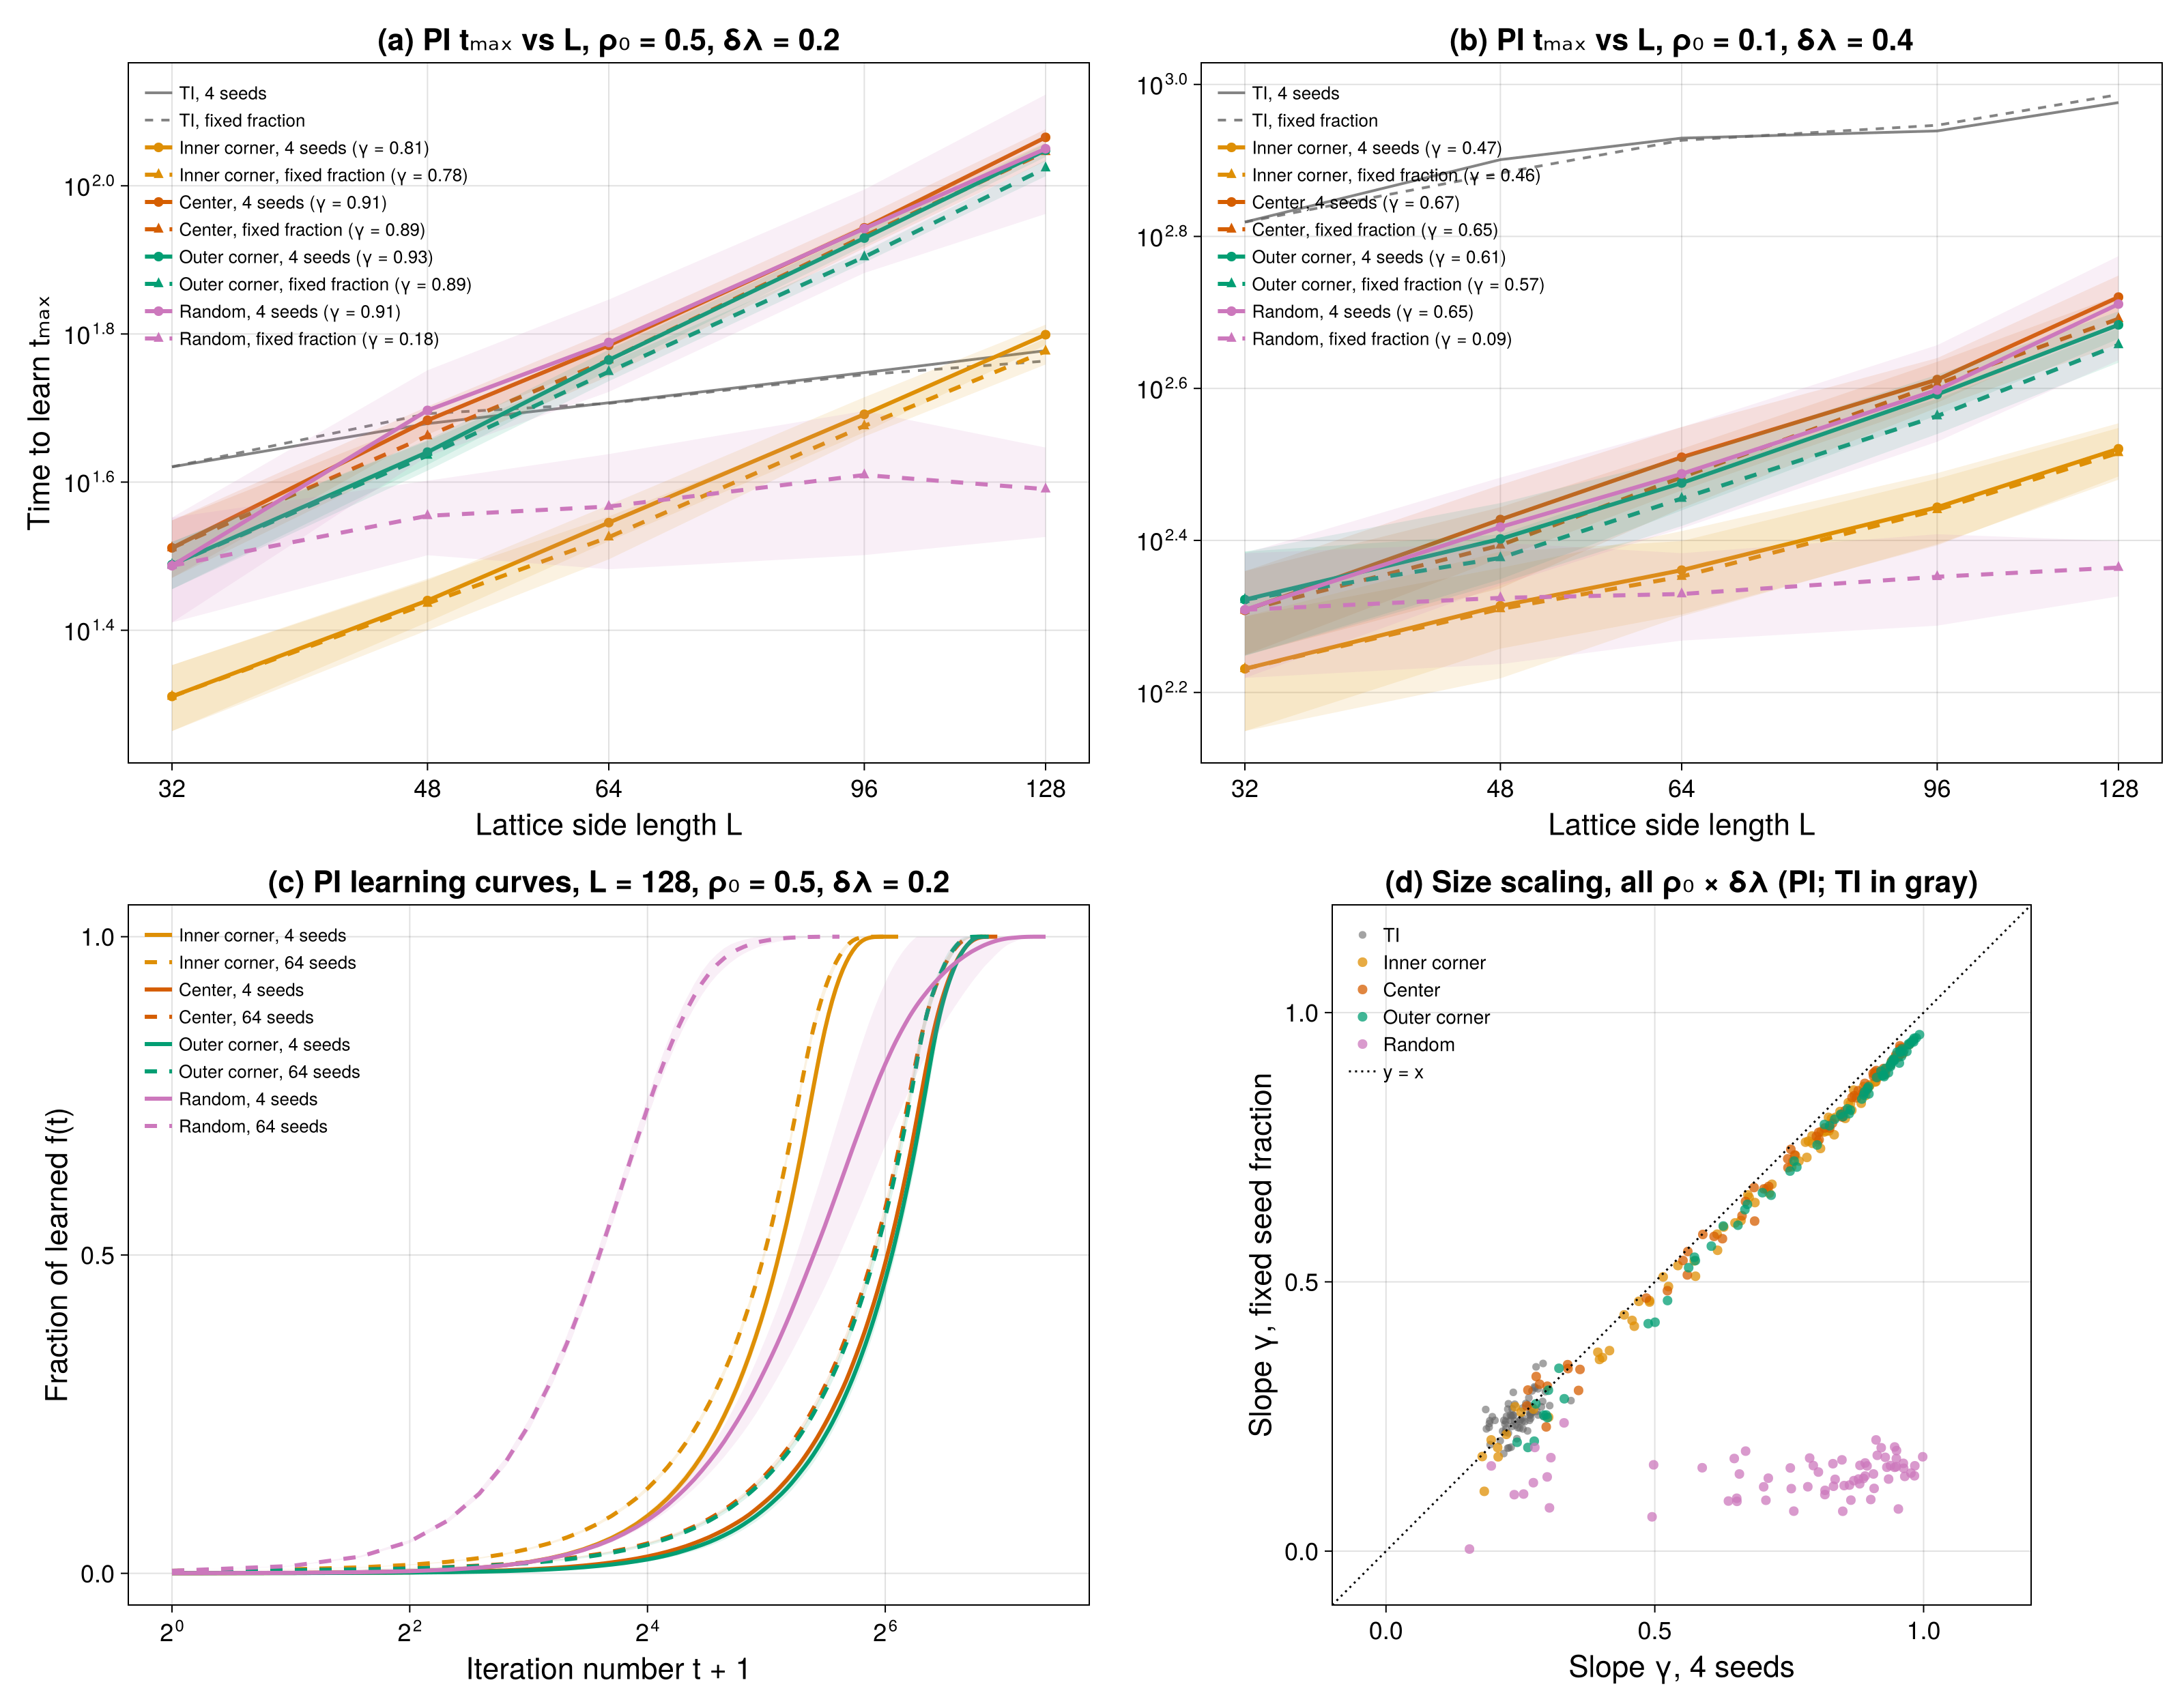
\includegraphics[width=\textwidth]{figs/figureC1.png}
    \caption{Size scaling of the nearest-neighbor regime with four initially learned agents (solid lines, circles) and with a fixed initial learned fraction (dashed lines, triangles).
    (a,~b)~$t_{\rm max}$ against lattice side $L$ (logarithmic axes) for each seating arrangement, at $\rho_0=0.5$, $\delta\lambda=0.2$ and at $\rho_0=0.1$, $\delta\lambda=0.4$; the broadcast regime is shown in gray, and the legends give the scaling exponents $\gamma$ (log--log slopes). Lines show the mean and bands one standard deviation over 20 runs.
    (c)~Nearest-neighbor learning curves at $L=128$ with $4$ and $64$ initially learned agents.
    (d)~Scaling exponent $\gamma$ with a fixed initial learned fraction against $\gamma$ with four initially learned agents, for every combination of $\rho_0$ and $\delta\lambda$; points on the dotted line $y=x$ indicate that the size dependence is unaffected by the number of initially learned agents.}
    \label{fig:seed density}
\end{figure}

% To print the credit authorship contribution details
\printcredits

%% Loading bibliography style file
%\bibliographystyle{model1-num-names}
\bibliographystyle{cas-model2-names}

% Loading bibliography database
\bibliography{cas-refs}

% Biography
%\bio{}
% Here goes the biography details.
%\endbio

%\bio{pic1}
% Here goes the biography details.
%\endbio

\end{document}

